\documentclass[a4paper, english, twoside, 12pt]{article}
\usepackage[margin=2cm]{geometry}
%The breakdowns for marking the report are as follows: 	
%	literature review/background (10%);
%	execution of the research project, quality of analysis, discussion of results (50%);
%	conclusions and value added (20%);
%	document presentation (20\%)

\usepackage{lmodern}	% Nice vector fonts
\usepackage{units}
% sets 25mm margins on A4
\setlength\textwidth{16cm}
\setlength\textheight{23cm}
\setlength\topmargin{-0.7cm}
\setlength\oddsidemargin{-0.6mm}
\setlength\evensidemargin{-0.6mm}
%\setlength\oddsidemargin{-0.3cm}
%\setlength\evensidemargin{0.3cm}
\renewcommand{\baselinestretch}{1.5}
\usepackage{float}

\usepackage{amsmath}
\usepackage[utf8]{inputenc}    %nice copy and pasting
\usepackage[T1]{fontenc}       %makes text copy-and-pastable
%\usepackage{natbib}            %for bibliography stuff
\usepackage{graphicx}          %for images
\usepackage{epstopdf} 			%To import unsw emblem and stuff
\usepackage{listings}
\usepackage[acronym, nomain]{glossaries}

\makeglossaries
\newacronym{set}{SET}{Single Electron Transistor}
\newacronym{cqc2t}{CQC2T}{Centre for Quantum Computation and Communication Technology}
\newacronym{pcie}{PCIe}{Peripheral Component Interconnect Express}
\newacronym{dma}{DMA}{Direct Memory Access}
\newacronym{adc}{ADC}{Analogue to Digital Converter}
\newacronym{fpga}{FPGA}{Field-Programmable Gate Array}

%\DeclareGraphicsExtensions{.eps}

\usepackage{wrapfig}           %for figures
%\usepackage[export]{adjustbox} %for putting boxes around figures
\usepackage{url}               %allow pretty formating of URLs \url{www.example.com}
\usepackage{booktabs}          % good tables package
\usepackage{multirow}          %merging table cells
\usepackage{varioref}          %for doing "table x on page y" with \vref{tab:label}
\usepackage{caption}           %to use minipage for inserting figures
\usepackage{float}             %for H figure and table placements Here.
\usepackage{pdfpages}          %To include pdfs
\usepackage[nottoc, notlot, notlof, numbib]{tocbibind} %Number the references section
\usepackage[title, titletoc, header]{appendix}
\usepackage{tikz}
\usepackage{braket}
%\usepackage{array}
%\newcolumntype{L}[1]{>{\raggedright\let\newline\\\arraybackslash\hspace{0pt}}m{#1}}
%\newcolumntype{C}[1]{>{\centering\let\newline\\\arraybackslash\hspace{0pt}}m{#1}}
%\newcolumntype{R}[1]{>{\raggedleft\let\newline\\\arraybackslash\hspace{0pt}}m{#1}}

\raggedbottom


%these 3 lines automatically render opening double quotes the right way around
%(They normally appear backwards)
\usepackage [english]{babel}
\usepackage [autostyle, english = american]{csquotes}
\MakeOuterQuote{"}
\usepackage{rotating}
\usepackage{subcaption}
\usepackage{pdfpages}

%\usepackage[colorinlistoftodos]{todonotes}%to do notes
\usepackage[disable]{todonotes} %Uncomment for the final version


\graphicspath{{./img/}}

%\setcounter{tocdepth}{2}% remove subsubsections from table of contents
   
%This package must go last, or it won't work
%With this package, you can click on cross references, URLs and page numbers, and you'll be taken there.
\usepackage[hidelinks,%clickable cross references and URLs, without visable formatting
            pdftex,%pdf meta data
            %pdfauthor={},%pdf meta data
            pdftitle={z3421023 Thesis A Report},%pdf meta data
            ]{hyperref}
            
%\linespread{1.25}
\begin{document}

\pagenumbering{roman}
%\includepdf{./src/cover_sheet.pdf}

%  Include the cover page
\newgeometry{margin=2cm}
\thispagestyle{empty}
\begin{center}
	\centering
\includegraphics[width=0.8\textwidth]{Arms-vl}\\
	[0.5cm]
\textbf{\large SCHOOL OF ELECTRICAL ENGINEERING\\
AND TELECOMMUNICATION}\\[2cm]
{\addtolength{\baselineskip}{0.5cm}
\textbf{\Huge
Ultra-High Fidelity Spin Qubit Initialization with Digital Feedback} \\[0.5cm]
}
{\Large by}\\[0.5cm]
\textit{\huge
Mark Johnson} \\[1.5cm]
{\Large
Interim Thesis A (ELEC4120) Report\\[2ex]
\vfill
Submitted: \today\hfill
Student ID: z3421023\\[-1.0ex]
Supervisor: Andrea Morello\hfill
Topic ID: AM5\\
\vspace*{-1cm}
}
\end{center}
\pagebreak

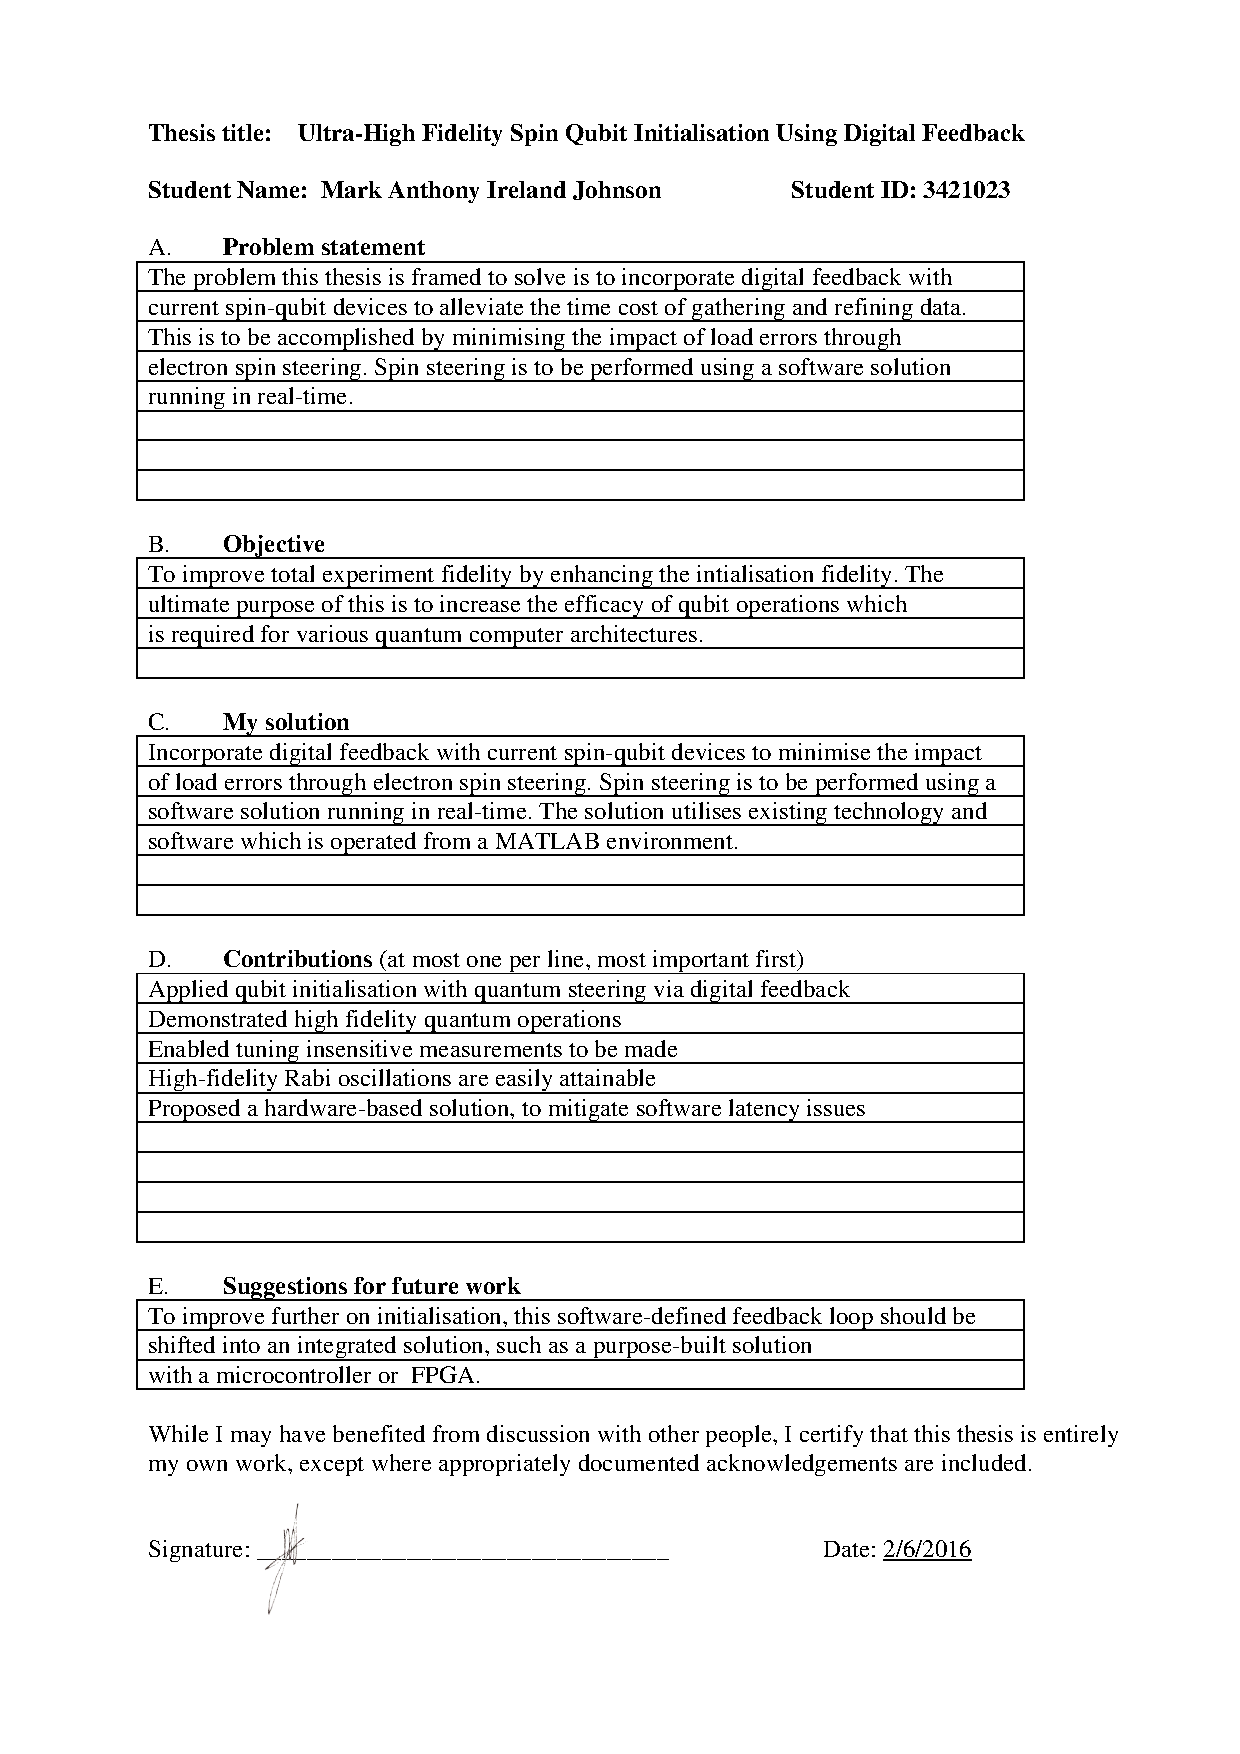
\includepdf[pages={1,2}]{./src/summary}
\pagebreak
\restoregeometry
\pagenumbering{arabic}

\listoftodos

\pagebreak

% Disable first glossary references in list of figures, or table of contents
\glsunsetall
\tableofcontents
\pagebreak
\listoffigures
% Resets glossary references
\glsresetall
\pagebreak

\section{Abstract}
Quantum computers present a new paradigm for solving various tasks. A general purpose quantum computer has been proved to exceed a classical computer in certain applications, such as sorting a database, and is inherently better at modelling quantum effects and performing simulations, which has large implications for the drug industry and chemical engineering broadly. This report aims to introduce the concept of a quantum computer, and current attempts at creating and controlling qubits, quantum bits of information. The body of work in this thesis is geared towards improving qubit state initialization fidelity, which would make all further experiments for efficient and cost effective. The prime way of improving initialization is to incorporate a feedback loop that will self-correct for any potential error before proceeding with any further operations on the qubit. Digital systems have been used to great effect in closing the loop, and this is the approach taken through this report.
\pagebreak
\section{Introduction}
Modern computing devices are becoming ever smaller, and to remain functional they must be engineered to combat the encroaching quantum effects at these scales, with increasing difficulty. Intel's current process incorporates a 14nm FET channel, as such the design of these FETs has been greatly changed to eliminate quantum effects. \cite{intel_process} In the near future, Intel will continue moving to a 10nm process which is presenting with further challenges. \cite{intel_future}

The trend in transistor miniaturisation has been dubbed "Moore's Law", following a prediction made by Gordon Moore, co-founder of Intel, in 1965. \cite{moore1965cramming}

\begin{quotation}
	"The complexity for minimum component costs has increased at a rate of roughly a factor of
	 two per year ... Certainly over the short term this rate
	can be expected to continue, if not to increase." 
\end{quotation}
 Despite the remarkable accuracy of this prediction, many believe \cite{end_of_Moore_1, end_of_Moore_2} the inevitable breakdown of this rule will take place as the physical limitations of creating such devices exponentially increases the start-up cost of manufacturing, as well as the cost of research and development.

However, this brick-wall has sparked research into alternative forms of computation. One such example, is a general purpose quantum computer. A quantum computer is unlike any classical computer, in the sense that its principles of operation are entirely based on quantum mechanics, as opposed to the classical electronics which modern computers are designed from. The difference between these paradigms cannot be understated, and one is not simply a replacement for the other. Despite the lack of a working quantum computer at this point in time, many researchers have spent time designing certain algorithms and processes that would run on such a machine, and analysing the benefits of the architecture compared to the classical computer. One such example is Grover's algorithm \cite{grover1996fast}, which is a method to sort databases which has a worst-case execution time of $\mathcal{O}(\sqrt{n})$, a remarkable improvement over the theoretical limit of any classical comparison based algorithm, $\mathcal{O}(n \log{n})$.


\todo[inline]{Introduce the work I'm doing, in particular. Describe structure of document}

\begin{figure}[htbp!]
	\centering
	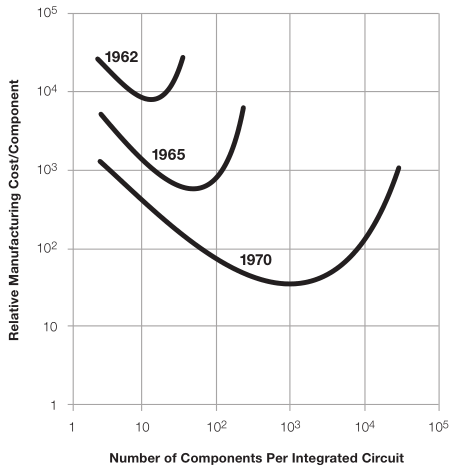
\includegraphics[width=0.8\textwidth]{moores_law}
	\caption{Gordon Moore's Prediction on Component Cost - Moore's Law}
	\label{fig::moores_law}
\end{figure}

\pagebreak
\section{Theory and Background}
\subsection{State of the Art}
% Review all of the current experimental evidence pertaining to my area of research
\todo[inline]{Talk quantum electron spin, projective measurement vs non-projective measurement (bloch sphere), about technology behind SETs}
\cite{nuclear_spin_readout}
\subsection{Devices}
\subsubsection{PCIe Digitizer Card}
\todo[inline]{Talking points of the Digitizer solution, DMA, etc. etc.}
%\subsubsection{FPGA/$\mu$Controller and ADC}
\todo[inline]{Talking points of the external FPGA and ADC solution, mention some particular examples of ADCs etc.}
\subsubsection{XMC}
\todo[inline]{Talking points of the integrated XMC solution, pre-built FPGA, ADCs and possibly with Auto-DMA}

\pagebreak
\section{Simulation}
\label{sec::simulation}
\subsection{Post-Processing Results}
	To verify MATLAB as a viable solution, it was first used against a full set of data that had been collected from a previous experiment. A set of 3 tests were performed, the first was to simply process the entire data in a single operation. This was the least like a real-world test, but served as a proof of concept that the peak detection, and time-out period were working. Once this was established, the next logical step was to perform this task on subsets, or windows, of the full data set. This is closer to a real test, and is actually extensible to the next alternative solution, as data processing on an embedded system can be limited by available memory. The test itself performed as expected, mirroring the first test. The final test was perhaps the most like a real-world solution, where a circular buffer of a fixed size (512 samples) is filled, which mimics a streaming input. This allows for a near-real-time time-out detection, supposing that the time it takes to process the signal is less than the time it takes to fill a time slice of the buffer (arbitrary, 32 samples in this example). Figure \ref{fig::timeout_detection} depicts the windowed solution in action over a large data set.
	
	\begin{figure}[htbp!]
		\centering
		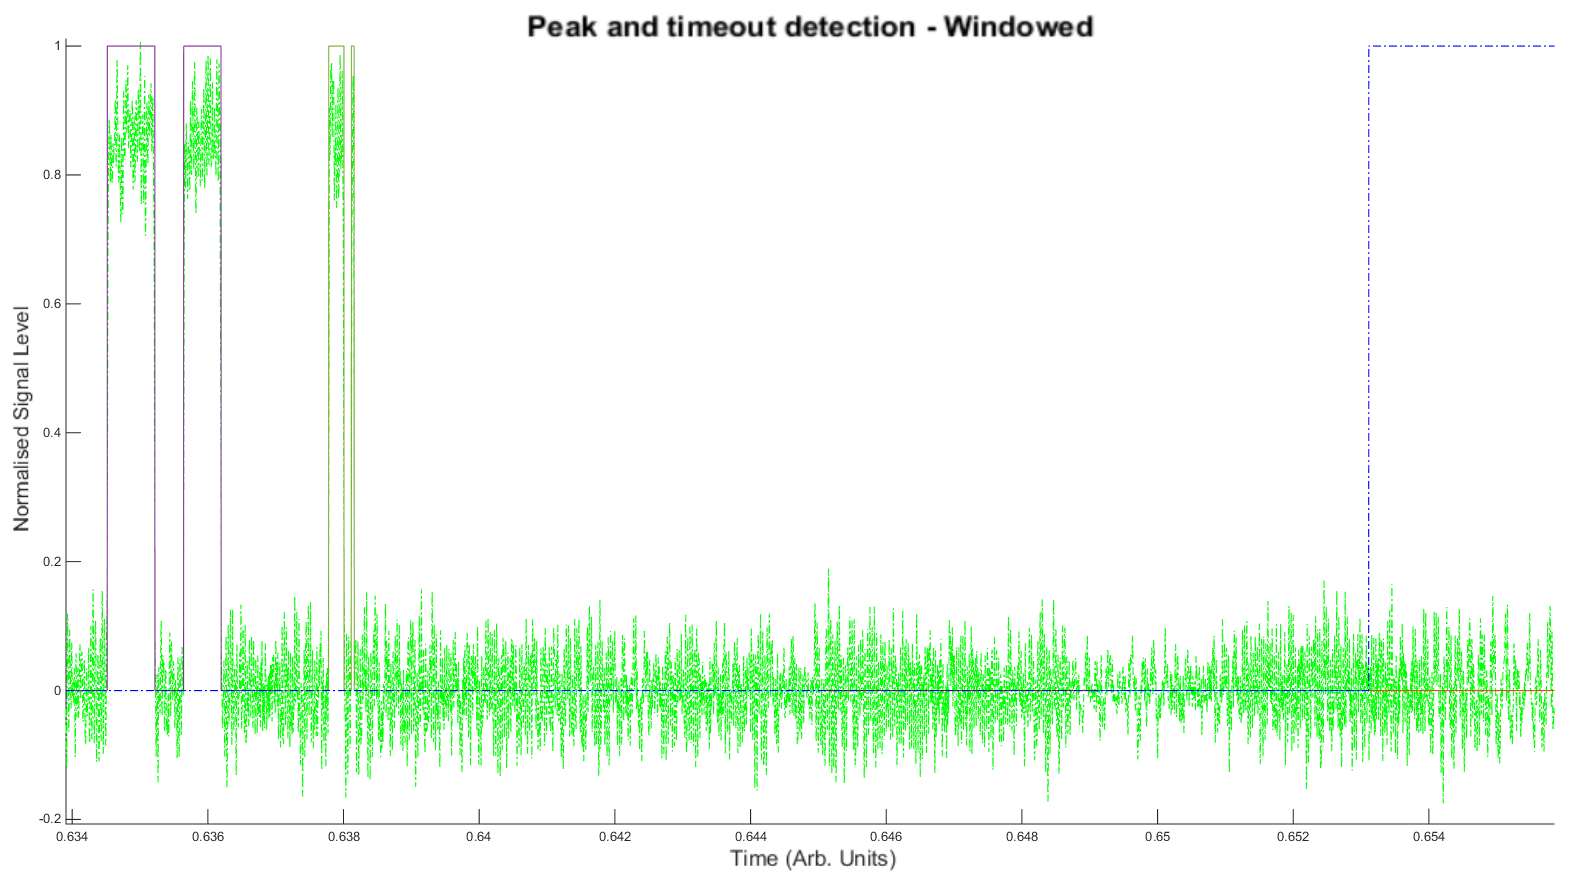
\includegraphics[width=\textwidth]{timeout_detection}
		\caption[MATLAB windowed peak detection on generated data]{MATLAB performing peak detection on windows of the green data set. The blue dashed line represents the output signal, once a set amount of time has passed}
		\label{fig::timeout_detection}
	\end{figure}

\pagebreak
\section{Real-time Processing}
\label{sec::real-time}
\subsection{Device under Test}
\label{sec::experiment}
\todo[inline]{Replace this section with Berdina}
Though experiments and designs are constantly evolving, at the core of this group's research is an \gls{set} used to perform electron spin readout. The apparatus I am applying my work to is by no means comprehensive, but it serves as a reference point in a proven device \cite{morello2010single}. To improve spin initialisation with this particular device would therefore be extensible to other devices and experiments.
Figure \ref{fig::thesis_experiment} shows a general layout used to control and read from an \gls{set}.

\begin{figure}[htbp!]
	\centering
	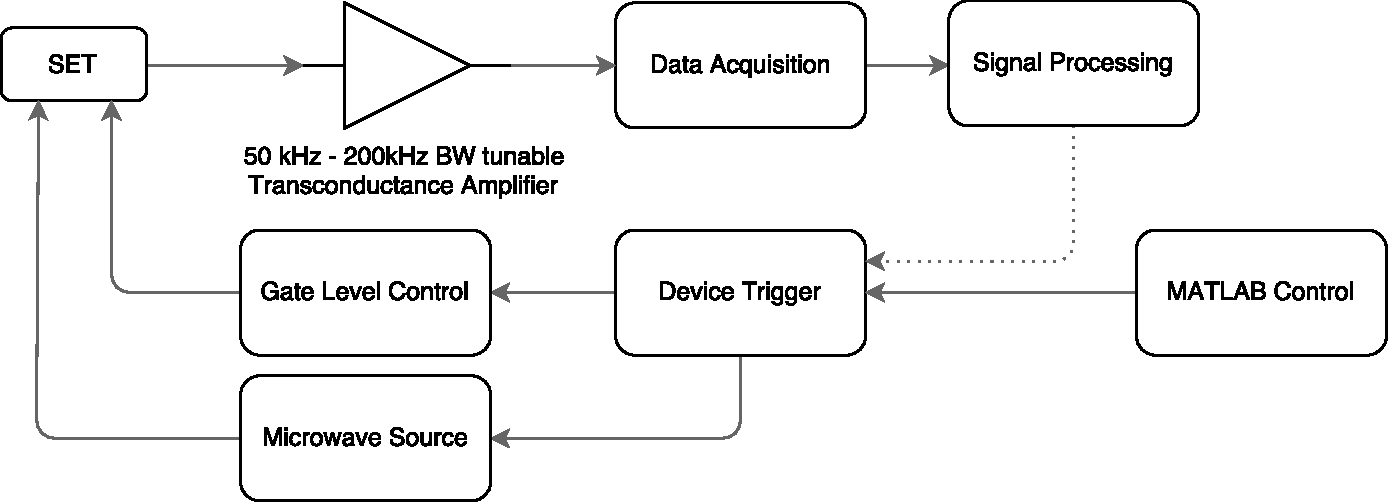
\includegraphics[width=\textwidth]{thesis_experiment.pdf}
	\caption{Block diagram of experiment}
	\label{fig::thesis_experiment}
\end{figure}


Figure \ref{fig::set_layout} shows the physical device that will be similar to one I will be testing my solution on. This devices has various voltage-controlled nodes, such as the top gate to induce a layer of electrons on the boundary, the left and right barriers to remove this layer, forming tunnel junctions to the island, and finally the plunger which can act at the gate as defined in section \ref{sec::set}.

\begin{figure}[htbp!]
	\centering
	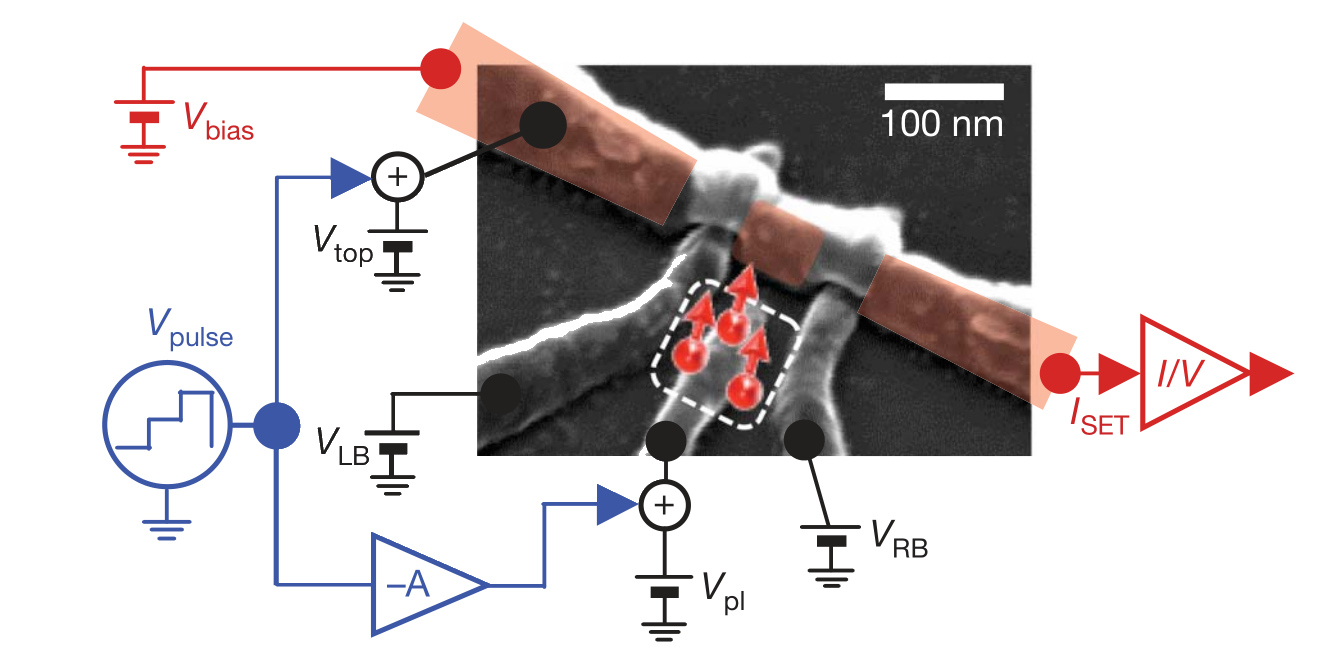
\includegraphics[width=\textwidth]{set_layout}
	\caption[Layout of an \gls{set}]{The layout of an \gls{set}\cite{morello2010single}}
	\label{fig::set_layout}
\end{figure}

\subsection{Set-Up and Equipment}
	\todo[inline]{perhaps explain here about the dilution refrigerator and the millikelvin environment}

\subsection{Experimental Procedure}

	\subsubsection{Gate Stimulus, NMR and ESR}
		To allow for precise control and measurement of the steering time applied to the electron donor, an electrostatic environment needed to be defined, along with radio and microwave stimulus. The \gls{set} donor is coupled capacitively to a number of gates, and so the tunnelling of an electron can be controlled simply by shifting the degenerate electron energy level about the Fermi level of the island. Once a magnetic field is applied, the degenerate electron energy levels split between the higher energy spin-up state, and the lower energy spin-down state. When tuned to the correct gate voltages, a spin-down electron's energy will be below the Fermi level, while a spin-up electron's energy will be above the Fermi energy, allowing tunnelling to unoccupied states. This is the ideal voltage to set our initialisation and readout levels. In Figure \ref{fig::sequence}, the \gls{set} control gate is being changed throughout the experiment, from empty to initialisation, then followed by a sequence of plunges and readouts. The plunge voltage will take the donor electron below the Fermi level, and so neither spin-state will be able to tunnel, as there are no available states in the reservoir, assuming the device is near absolute zero.
		
		
		\begin{figure}[htbp!]
			\centering
			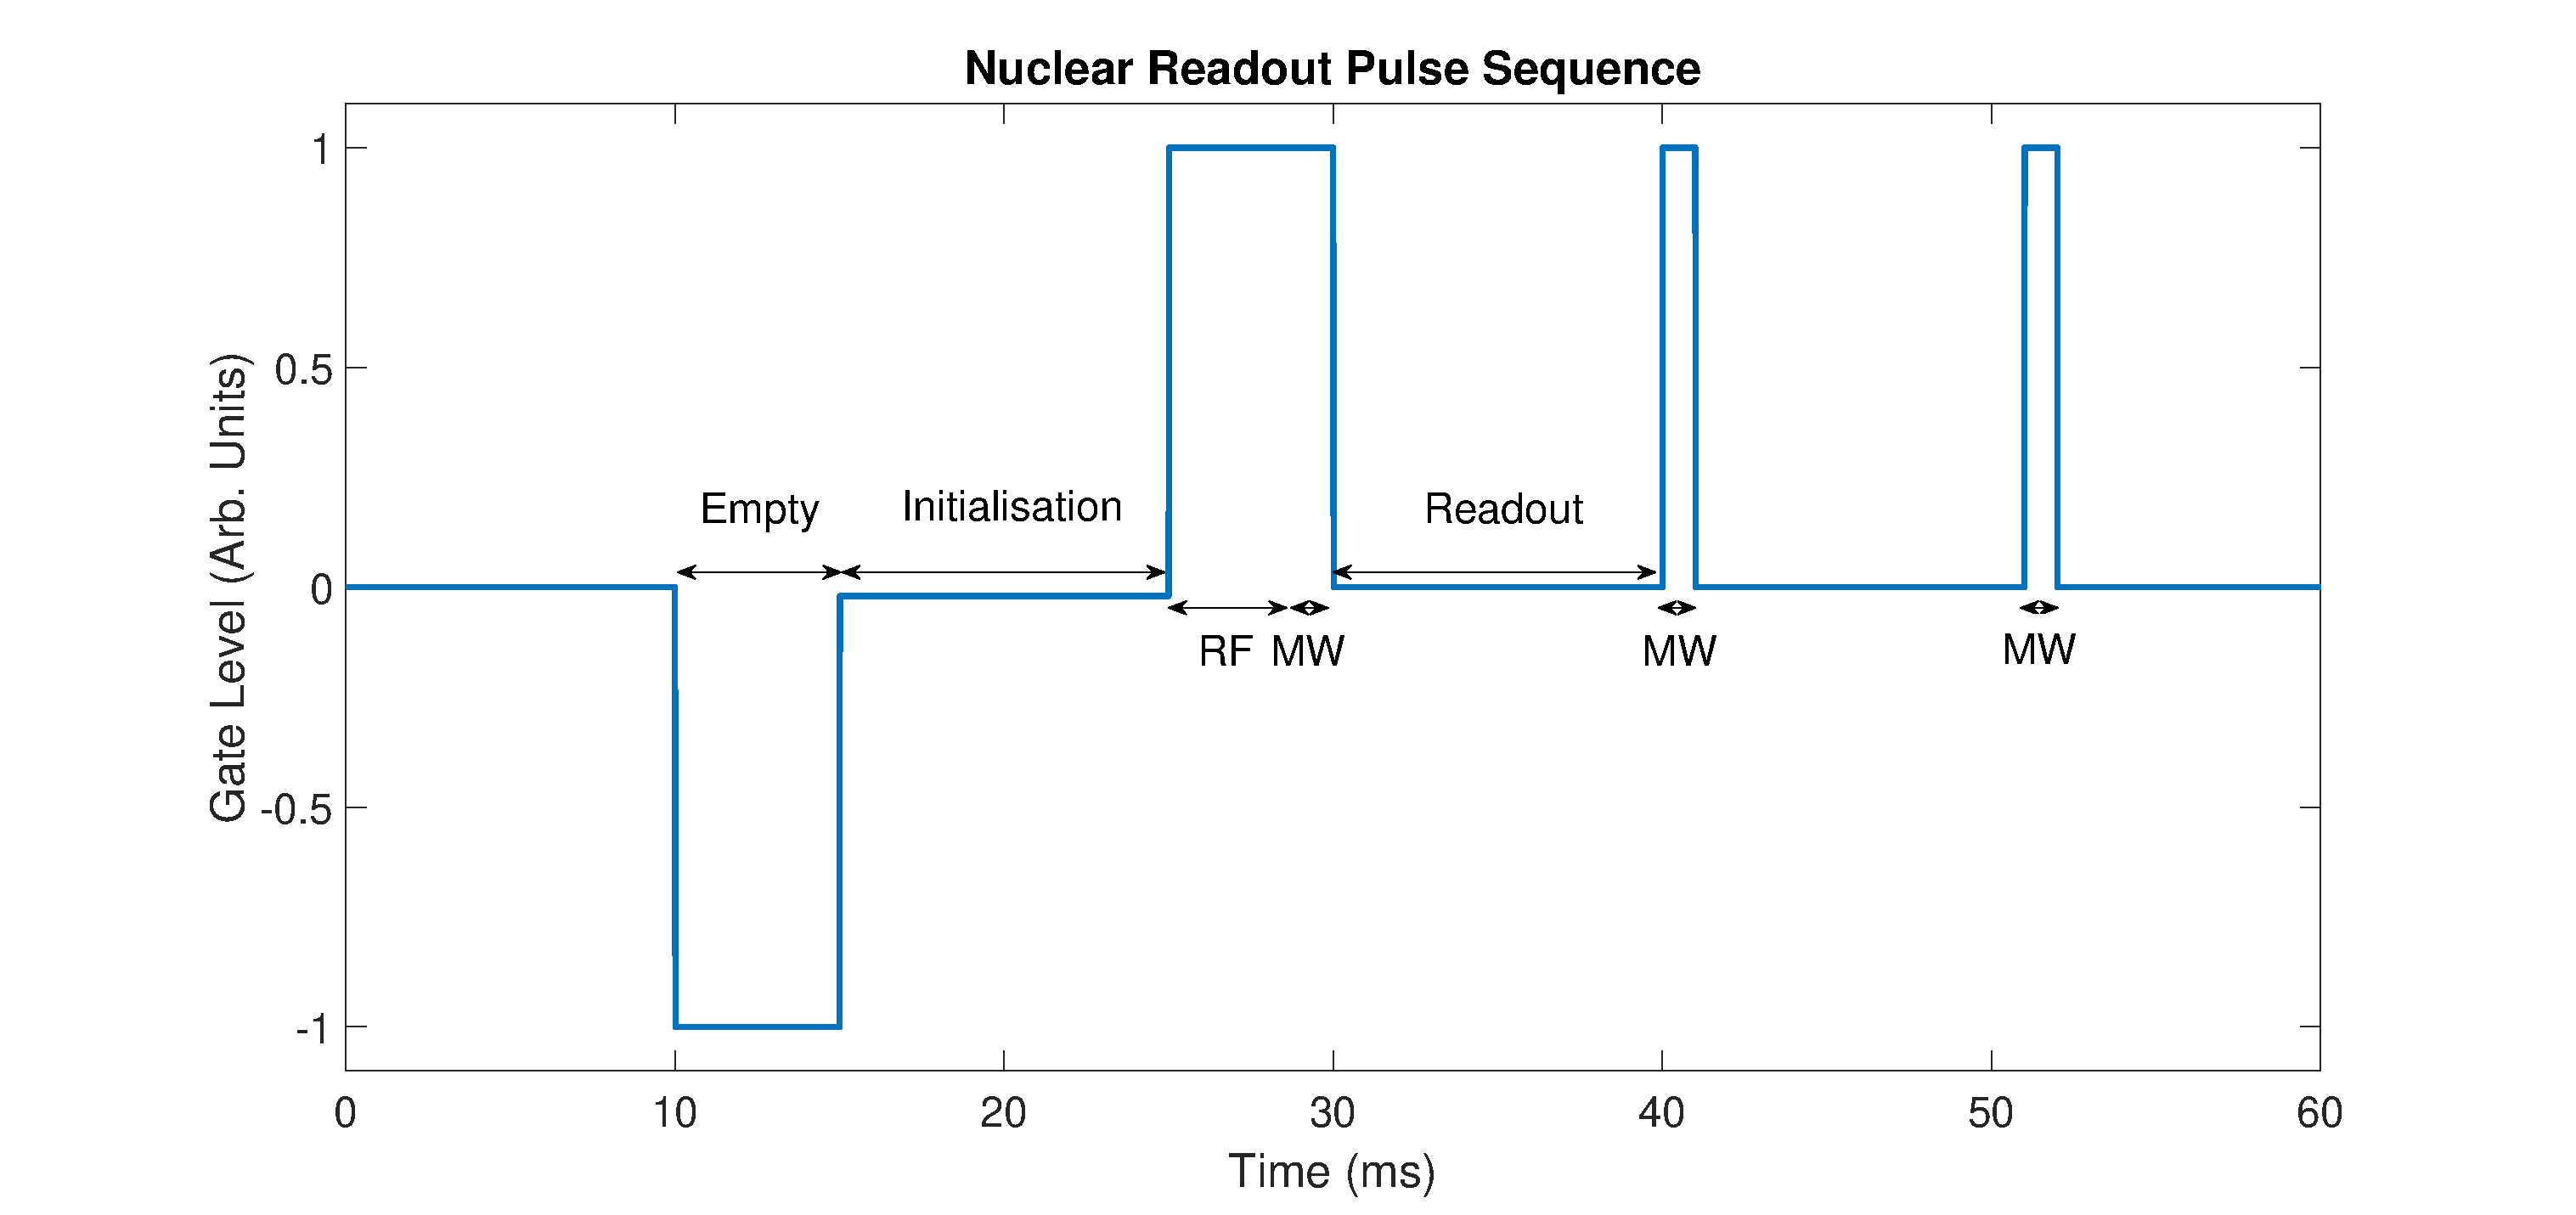
\includegraphics[width=\textwidth]{sequenceFigure}
			\caption{The control sequence, describing both gate levels as well as \gls{rf} and \gls{mw} stimulus, applied for this experiment.}
			\label{fig::sequence}
		\end{figure}
		
		During the initial plunge, a \gls{rf} pulse and a \gls{mw} pulse will be applied, to map the state of the donor electron to the nucleus and then to map the state of the nucleus to the electron, respectively. Mapping from nucleus to electron place during this stage is a short-hand method of beginning the readout phase, without first returning to the readout level.
		
		These \gls{rf} and \gls{mw} pulses are applying \gls{nmr} and \gls{esr}, conditional upon the state of the electron, for \gls{nmr}, and conditional on the state of the nucleus, for \gls{esr}. This is best explained by Figure \ref{fig::spin_levels}, where the state transitions are shown to require distinct driving frequencies, $\nu_{e1}, \nu_{e2}, \nu_{n1} \textrm{ and } \nu_{n2}$. Since the electron spin is expected to be spin-down when the \gls{rf} pulse is performed, the driving frequency to perform \gls{nmr} will be $\nu_{n2}$. Using this method we will perform a $\pi$-pulse, which will flip the nucleus state from spin-up to spin-down, or vice versa given that is in initially in one of these states. For each consecutive readout, the nucleus is expected to flip, as ideally each time a spin-down electron is loaded followed by a successful $\pi$-pulse.
		
		Once the nuclear state has been prepared, the sequence of electron state mapping and readout commences, which performs \gls{esr} conditional upon the state of the nucleus. The driving frequency for this transition is $\nu_{e2}$, so the readout phases should show tunnel events if the nucleus is spin-up.
	
		This measurement is repeated 20 times, to determine the state of the nucleus accurately, and then the experiment is repeated a set number of times (for the data presented in this report, the nuclear readout was performed between 500 and 2000 times). 
		
	\subsubsection{Magnetic Field Variation}
		Once the characteristics of quantum steering are established at a set magnetic field, it will be worthwhile studying the impact of this approach at lower magnetic fields. Lower magnetic fields incur more initialisation errors due to a smaller Zeeman splitting than with a higher magnetic field. If there is little affect on the efficacy of quantum steering for initialisation, and also on the readout fidelity, then a spin device can become far more practicable, as the level of \gls{esr} control is much simpler at lower driving frequencies, and often there are simply more numerous devices available at lower frequencies. The primary fields of consideration are 1.4 T, 1.0 T, and 0.7 T, which correspond to \gls{esr} frequencies  $\nu_{e1}, \nu_{e2} \approx$ 39 GHz, 28 GHz and 20 GHz, respectively.
		
		Furthermore, once the magnetic field on the Z-axis is below 1.0 T, we are able to define a full 3-dimensional magnetic environment using 2-dimensional vector magnets in the XY-plane, perpendicular to the large magnetic field described above. 1.0 T is the limit of these vector magnets, and as such full 3-dimensional control is impossible above this threshold.
		\todo{tie this together nicely...}
		
	
\pagebreak
\section{Results}
\label{sec::results}
\subsection{Quantum Steering Efficacy}
	\label{sec::steering}
\todo[inline]{Discuss all results related to nuclear spin mapping}

	As discussed in \hyperref[sec::nuc_spin_map]{section \ref{sec::nuc_spin_map}}, nuclear spin mapping was used to improve the readout fidelity of our experiment. However, the improvement in fidelity was conditional upon the initial state of the electron at the time of the mapping. To perform correct mapping, a spin-down electron is required. To measure the fidelity of the nuclear mapping, and implicitly the quantum steering efficacy, the state of the nucleus was measured for many steering times, and repeated to minimise the limits of accuracy in the measurement. Figure \ref{fig::wait_time} shows the total experimental error as a function of steering time. As steering time increases, we are more confident that the state of the electron was spin-down at the time of mapping, which is reflected in our decrease in error. The average time spent in the initialisation period is plotted on the right-axis. This would exceed the steering time in the average case, as a blip in current would require postponement of the donor plunge.	There are 2 separate data sets plotted, one each for $B = 1.4$ T and $B = 1$. For $B = 1.4$ T, there were 2001 nuclear readouts per data point and for $B = 1.0$ T there were 501 nuclear readouts.
	
	\begin{figure}[htbp!]
		\centering
		\vspace{-1cm}
		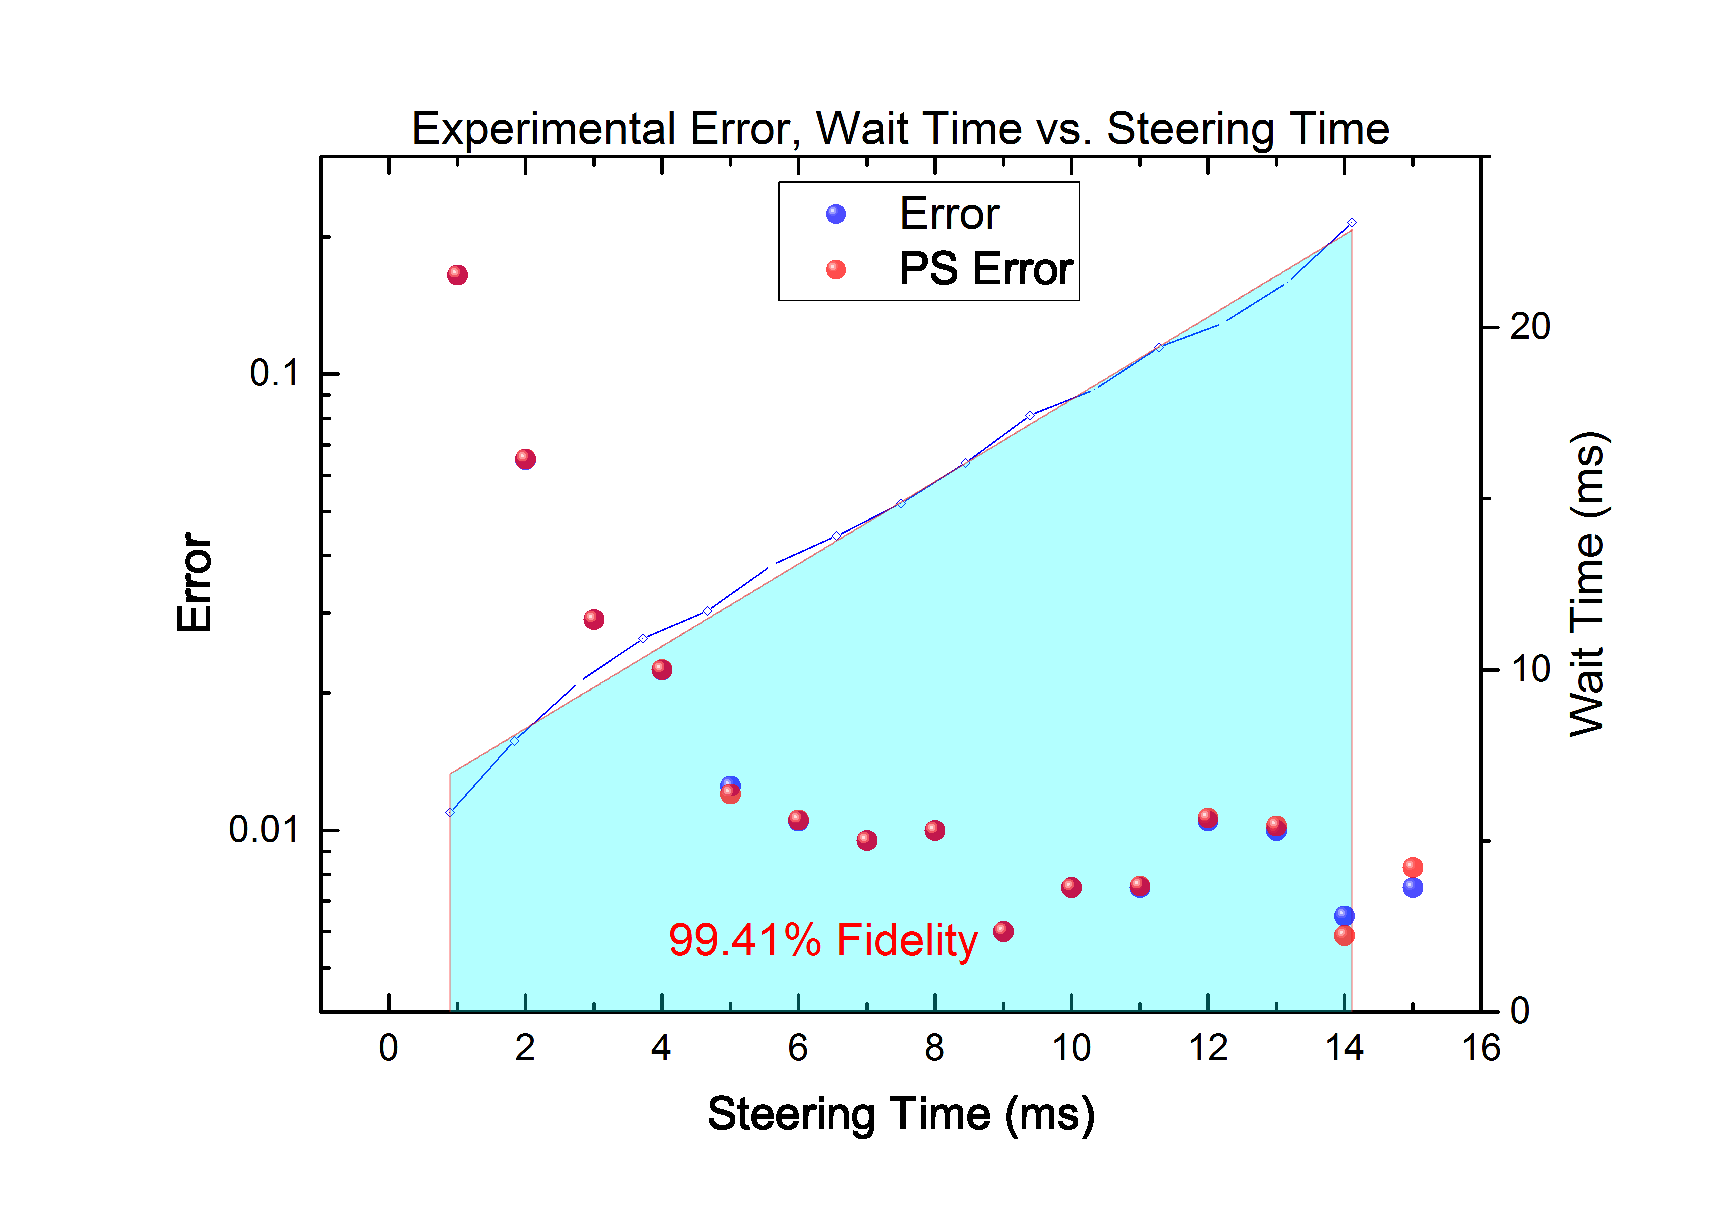
\includegraphics[width=\textwidth]{WaitTimeFigLog_1p4T}
		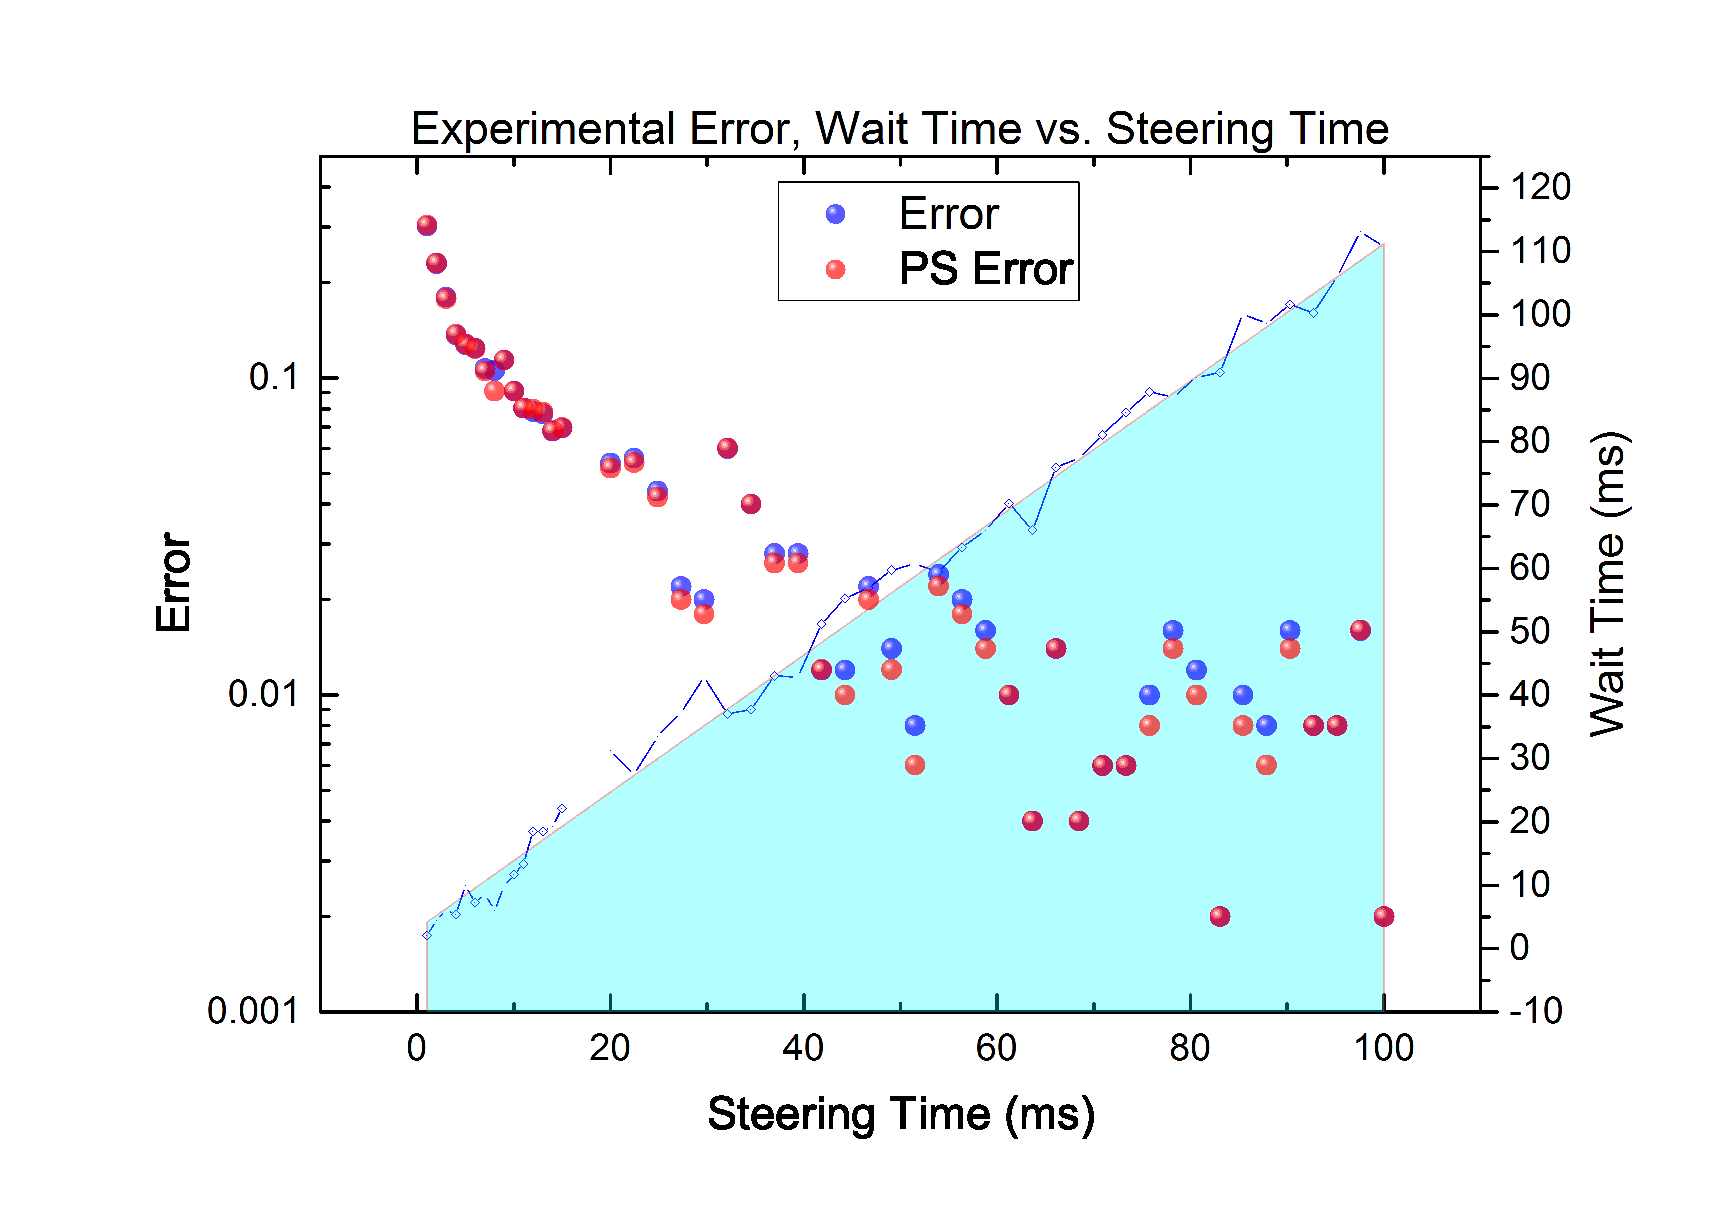
\includegraphics[width=\textwidth]{WaitTimeFigLog_1p0T}
		\caption[Experimental fidelity with varying steering times.]{For a field of $B = 1.4$ T (top) and $B = 1.0$ T (bottom), the experimental error is plotted against steering time. On  the right axis is the average time spent at the initialisation level during the experiment.}
		\label{fig::wait_time}
	\end{figure}
		
	These two datasets show the relationship between the required steering time for a good initialisation and the apparent tunnelling time of the donor electron. As expected, with a larger steering time the fidelity of the experiment approaches 100\% following an exponential decay, determined by the characteristic tunnel time. In each plot of Figure \ref{fig::wait_time}, there are two sets of points plotted, raw error data given by analysing all nuclear flips and post-selection (PS) error, where readouts that were initialised poorly are ignored. Poor initialisation will be explained and explored in \hyperref[sec::latency]{Section \ref{sec::latency}}. Post-selecting improves the experimental fidelity, as we remove cases which are likely to be cause an incorrect nuclear mapping, and it has been shown that with post-selection the experimental fidelity can reach 99.9\%, though, in these plots, the maximum is constrained by the limits of accuracy for the measurement, which was 0.2\% (500 readouts), and hence the maximum observed fidelity is 99.8\%. %\todo{somehow give citation to Stef, no paper on this though}

	This result exactly demonstrates the effect of quantum steering as a method for filtering incorrect initialisation through quantum-back action. The results mirror those presented in Section \ref{sec::spin_init}.
	
	The required steering time to achieve 99\% fidelity is much longer for $B = 1$ T, however it was observed that the average tunnel time had not significantly increased by such a margin from $B = 1.4$ T. This could be explained if we accept that the probability of a spin-down electron tunnelling off during the initialisation phase is high (also known as a dark-count), which is physically the same as a read-error. Whilst this is a possible explanation, it's not clear if this is accurate, and more examination of the data is required. All approximations made of a simple exponential decay have assumed that the dark-counts are negligible.

\subsection{Nuclear Rabi Oscillations}
%	\todo[inline]{Discuss results pertaining to a high fidelity readout from a nuclear/electron rabi}
	A nuclear Rabi oscillation was performed by loading an electron onto the donor, followed my mapping the state onto the nucleus. This electron is ideally spin-down for this step. After the nucleus is prepared, we stimulate it with an \gls{rf} pulse of duration $\tau_{RF}$, which is swept as part of the experiment. After the \gls{rf} exposure, we then map the nucleus state back onto an electron using another \gls{mw} pulse, followed by a readout of the electron state. We perform 20 repeated measures of the nuclear state via the electron in this manner. 	Figure \ref{fig::nuclear_rabi} shows the results of two separate Rabi experiments run back-to-back, one with electron initialisation by steering, and one without.
	
	
	As we vary $\tau_{RF}$, we observe that the expected value of the nuclear-spin readout, via the electron readout, follows a sinusoid with a frequency known as the Rabi frequency. Arbitrary rotations are a key part of a universal quantum computer, and naturally improving the initialisation fidelity can enable more accurate rotations.
	
	\begin{figure}[H]
		\centering
		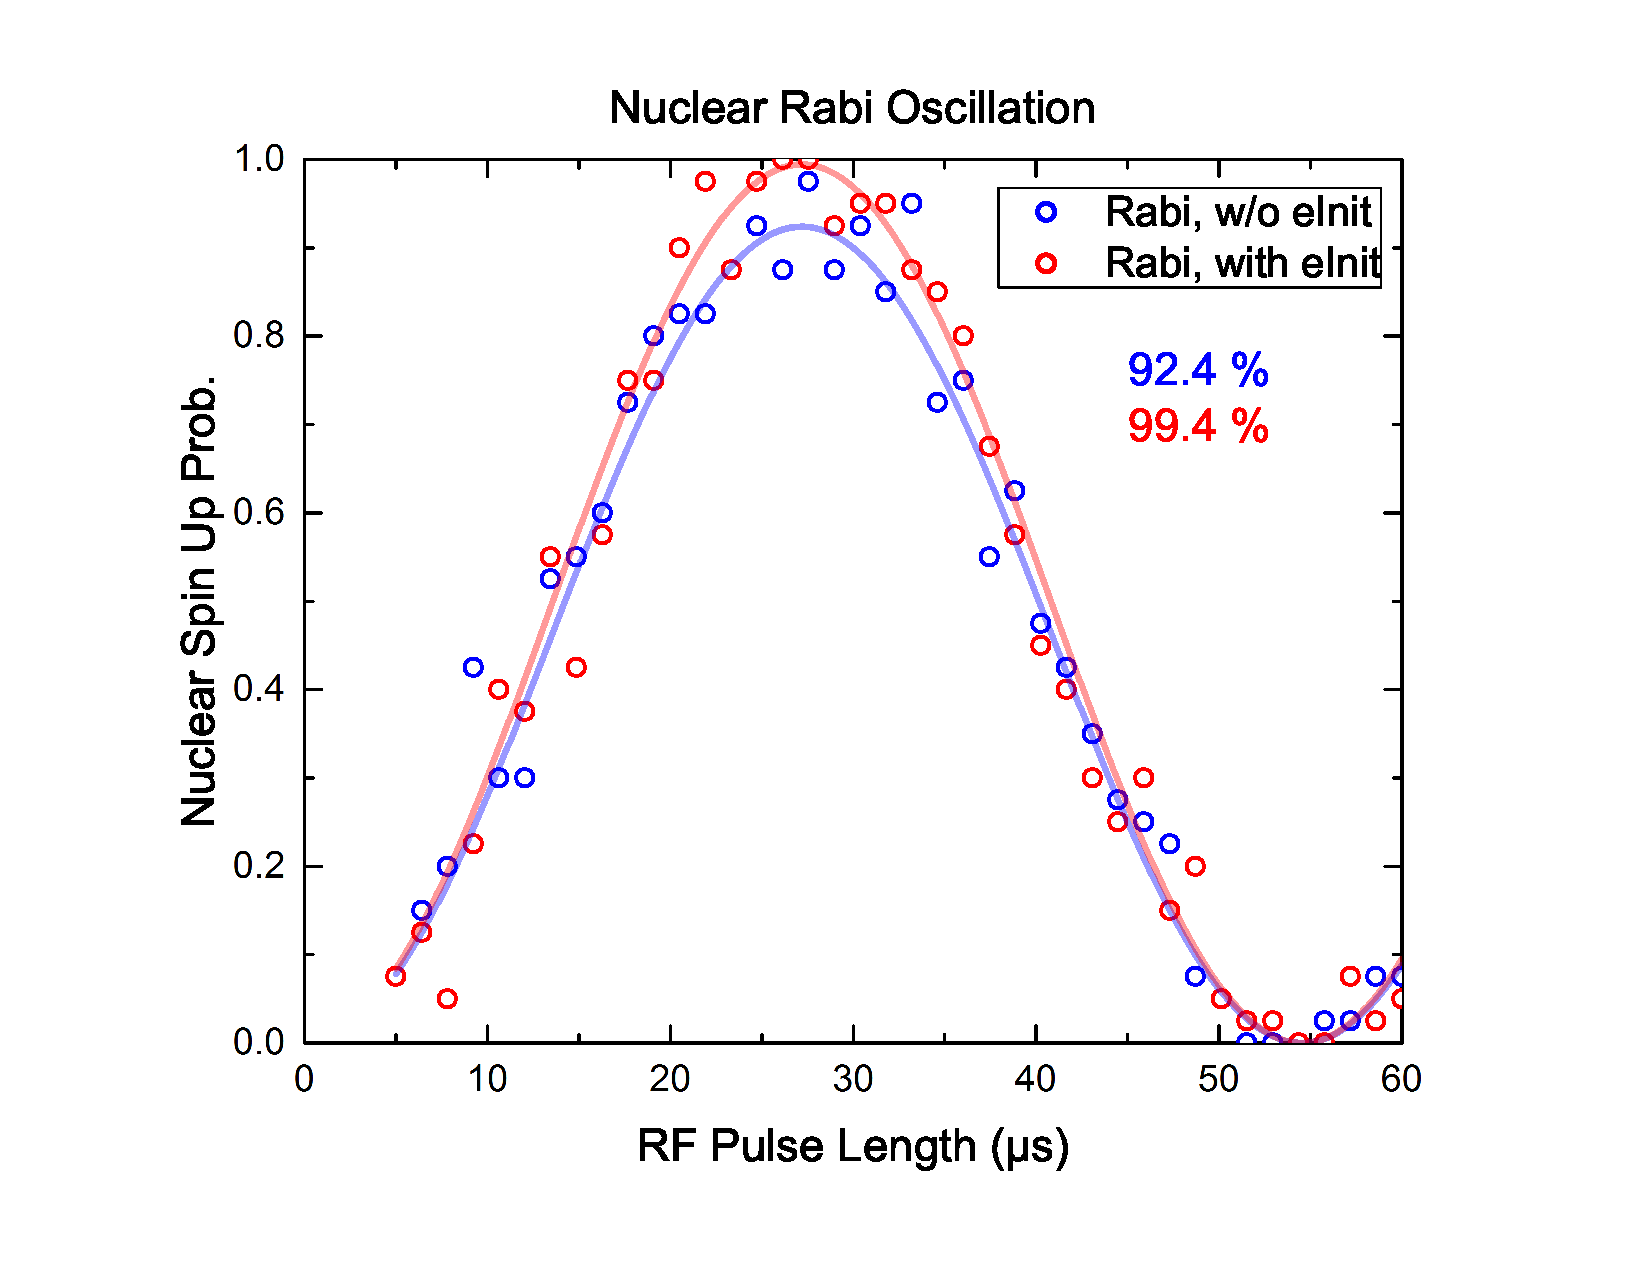
\includegraphics[width=0.8\textwidth]{nRabiFig}
		\caption{A nuclear Rabi oscillation with and without electron initialisation.}
		\label{fig::nuclear_rabi}
	\end{figure}
	
	If we have poor initialisation, this will affect the fidelity of our readout and would reduce the height of the peaks, as shown by the maximum of the fitted sine wave reaching only 92.4\% without initialisation, compared to 99.4\% with initialisation.

\subsection{Initialisation Level Tuning}
	The initialisation level of the pulse sequence was tuned to find the best position for a high fidelity experiment. It was discovered, however, that with initialisation there was a broad  flat-band (approximately 400 mV) in which high fidelity results were obtained. This indicates another benefit in performing electron initialisation, which is insensitivity to tuning. This is a very useful property for a quantum computer, as reproducibility of measurements is crucial in determining the result of a computation.
	
	Figure \ref{fig::initLevel} shows the error rate as a function of initialisation level. As the initialisation level changes, the donor potential will also change with respect to the Fermi level of the reservoir, leading to changes in load and read errors, as explained in Section \ref{sec::load_error}. To reiterate, if the potential of both a spin-up and spin-down electron is such that both have available energy states in the reservoir, they can both tunnel out. If the Zeeman splitting of the donors is much larger than the thermal energy of the system, then we would expect a fairly large region in which to tune the initialisation level, while maintaining spin-dependent tunnelling. 
%	Typically, $ k_B T \ll h \nu_{e2}$, where $k_B, T$ are Boltzmann's constant and the device temperature, respectively.
	By sweeping the initialisation level we observe a cut-off region, greater than approximately 0 V, where the experimental fidelity drops completely. On the negative end of the scale, there appears to be an exponential drop in fidelity, as read errors begin to occur more frequently. Read errors increase as a negative bias shifts the donor potential above the Fermi level, bringing more available states to the level of a spin-down electron.
	
	It is expected that if the steering time is increased, the drop off due to increasing read-errors will diminish, as the steering window will filter more tunnel events. This has not been explored in this thesis due to lack of measurement time.
	
	\begin{figure}[htbp!]
		\flushleft
		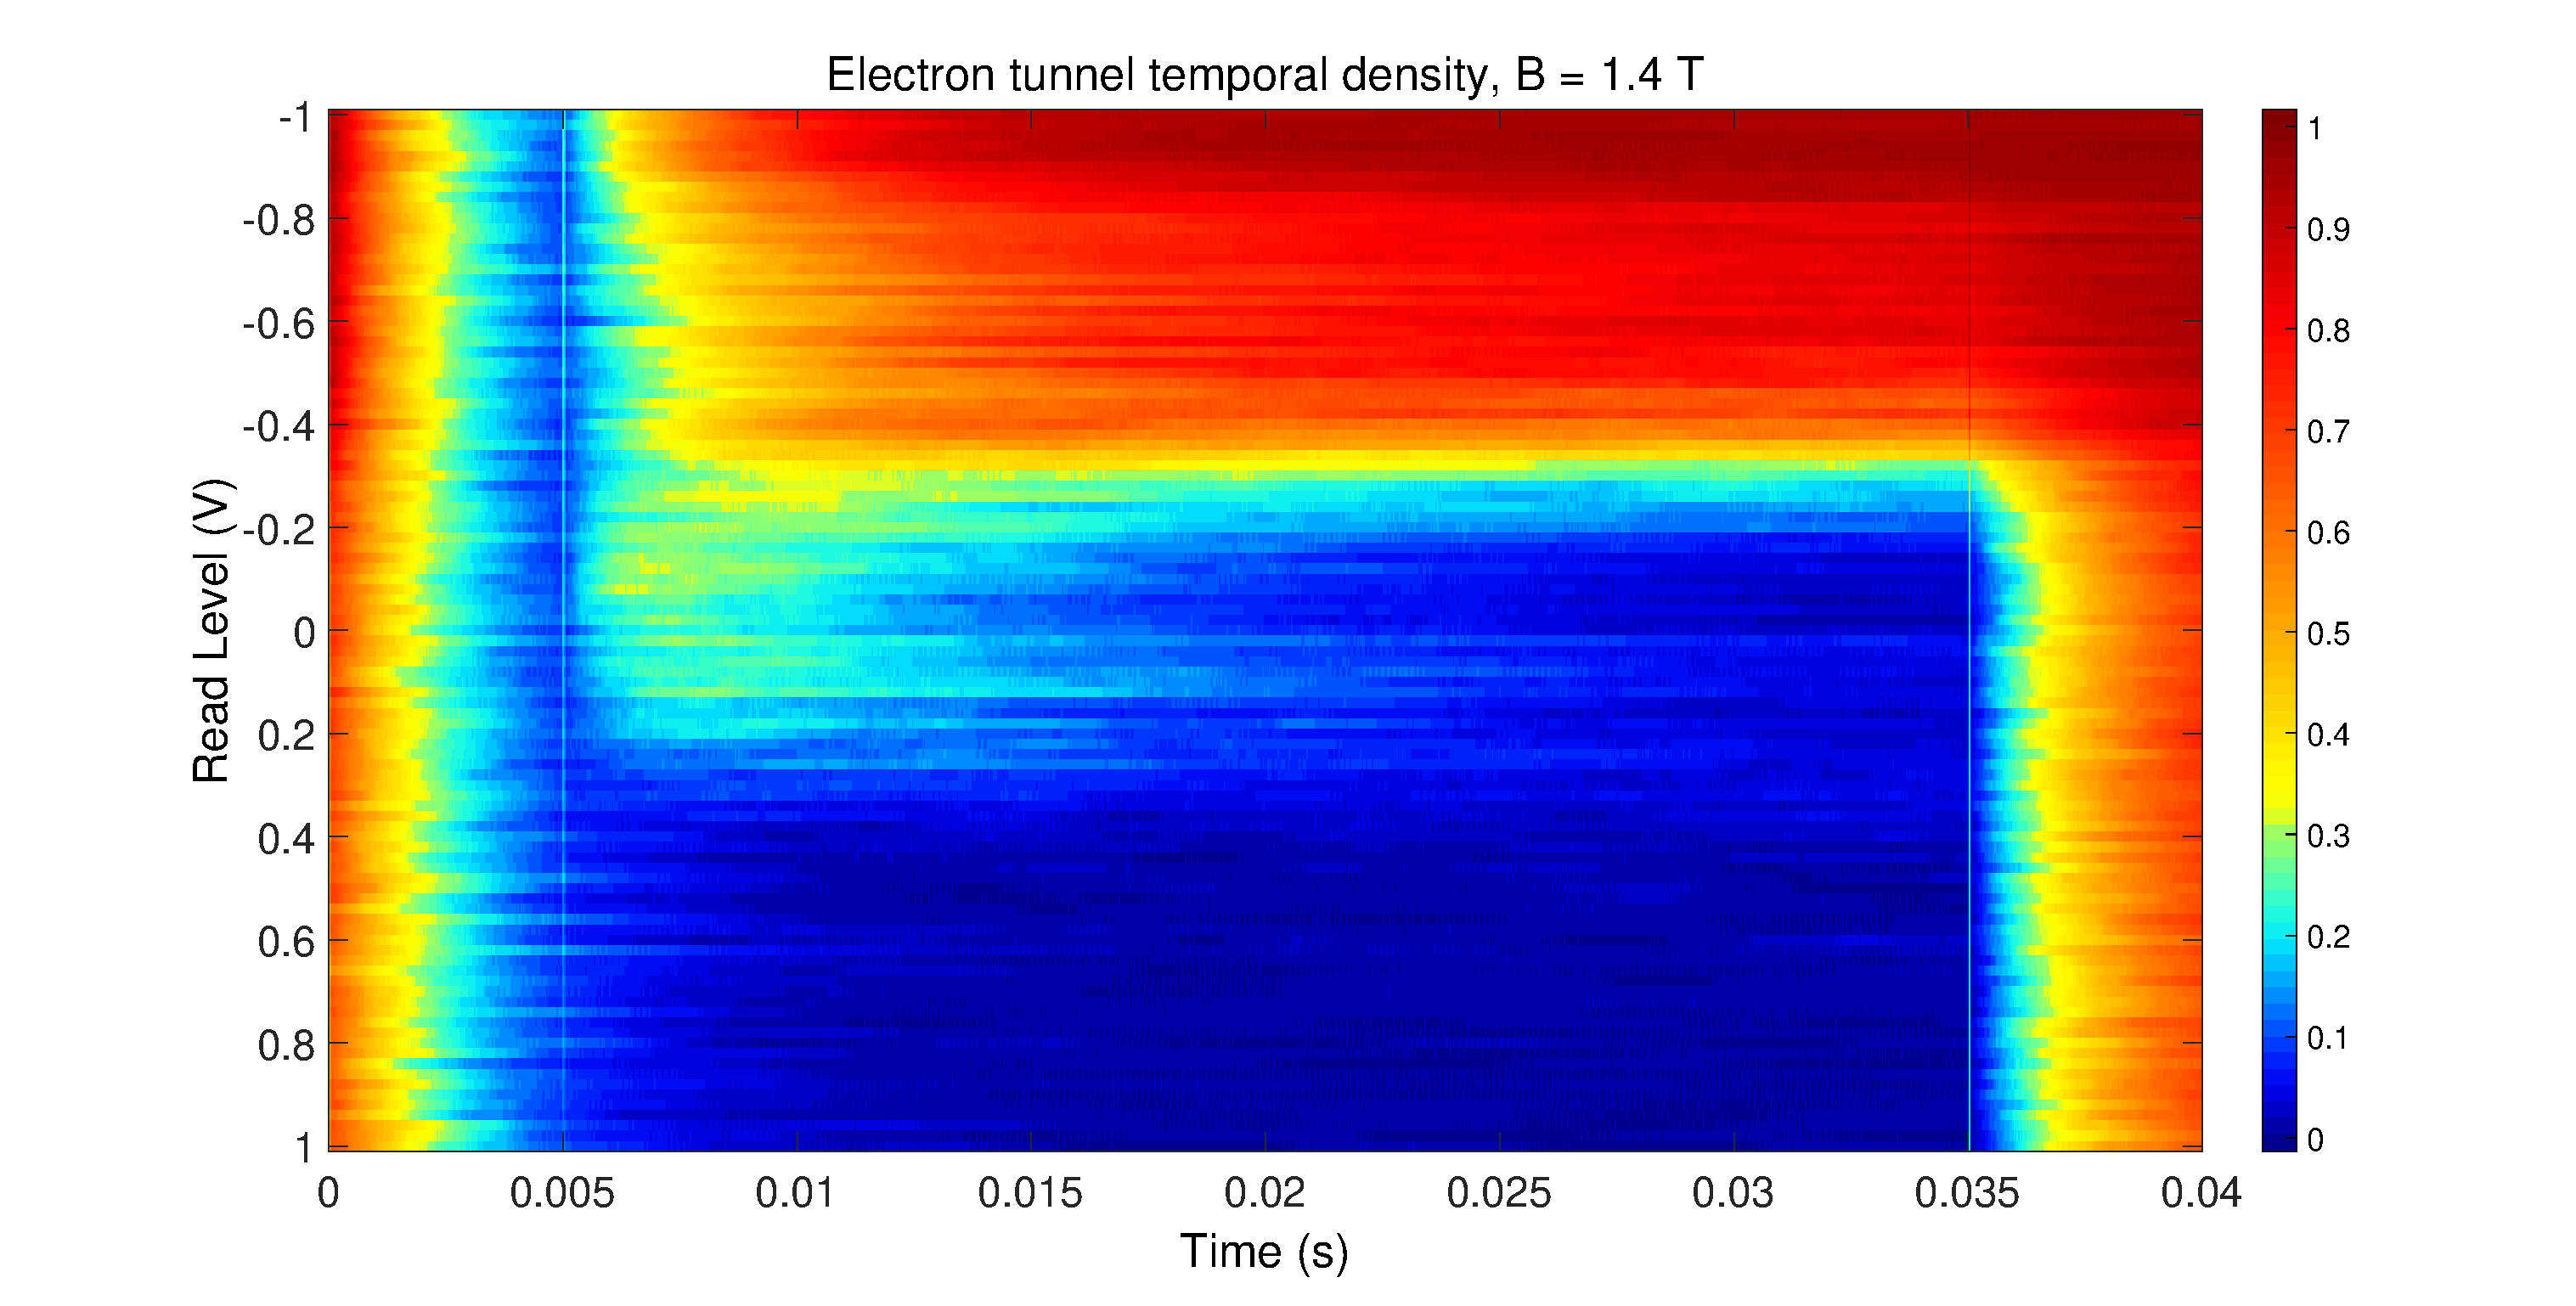
\includegraphics[width=\textwidth,height=0.4\textheight]{readLevelScan_1p4T}
		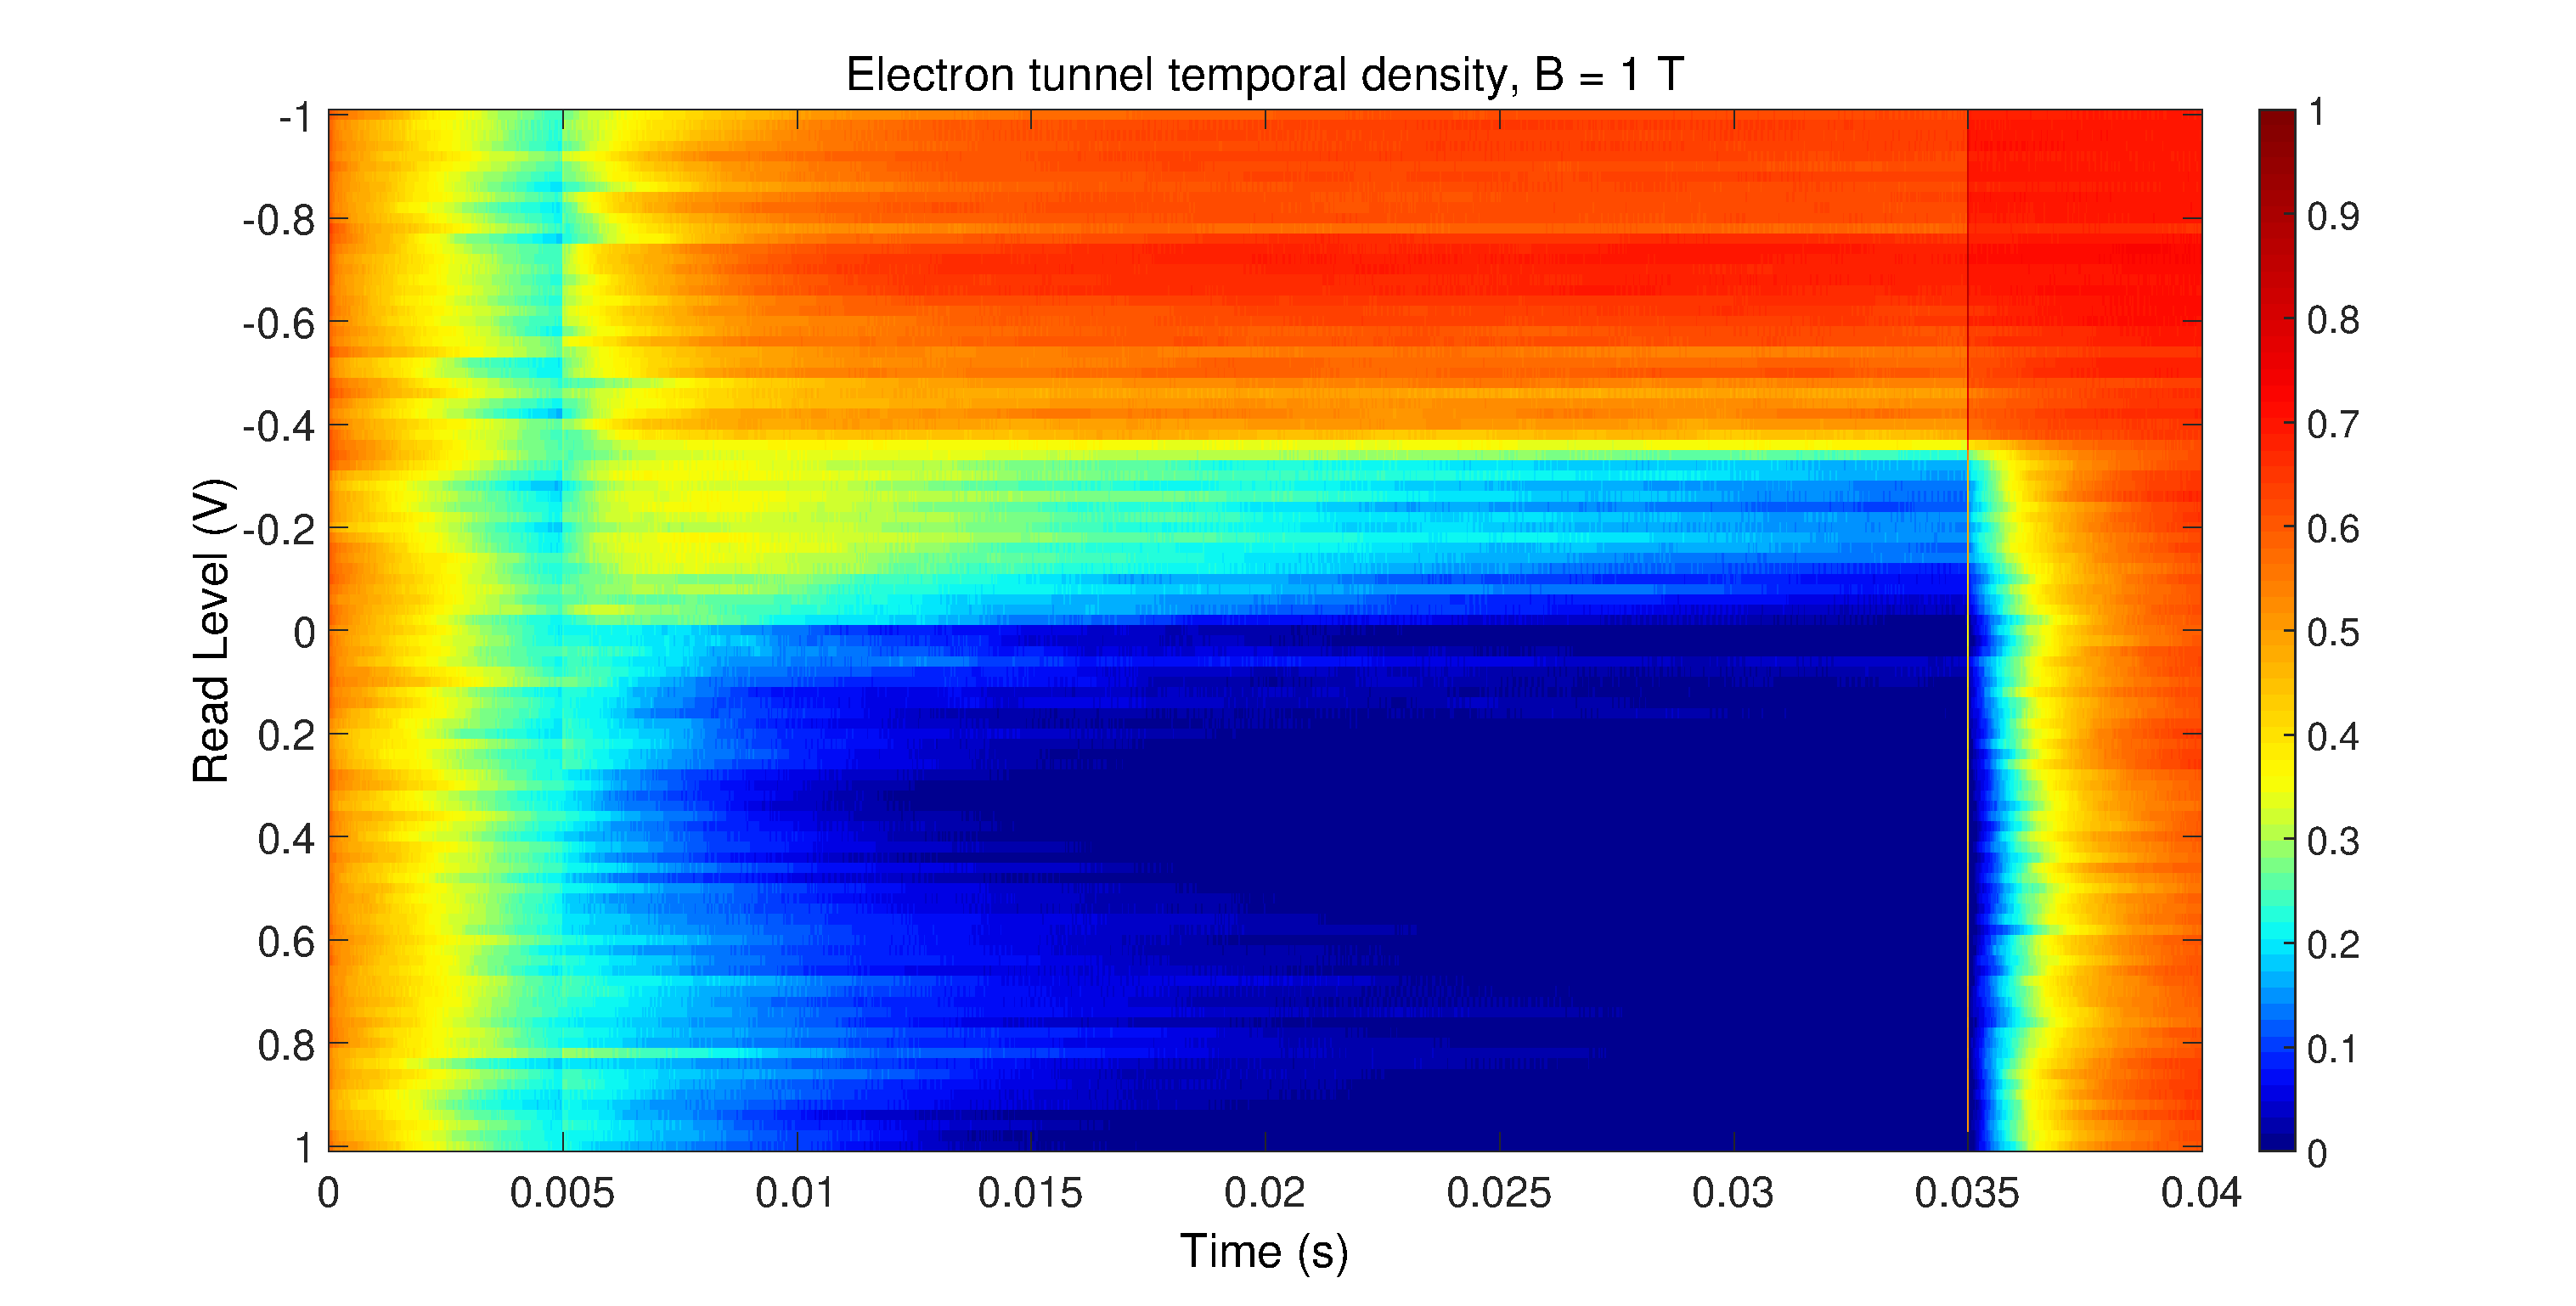
\includegraphics[width=\textwidth,height=0.4\textheight]{readLevelScan_1p0T}
		\caption[Read level scan for two magnetic biases]{For a field of $B = 1.4$ T (top) and $B = 1.0$ T (bottom), the tail of a read level scan is plotted, where red indicates a high current through the \gls{set} while blue indicates low current. The values are averaged over many runs. 
		Above a certain threshold, the donor will remain ionised and current will continue to flow throughout the load-read-empty cycle. Below a certain threshold the opposite will occur, where any electron on the donor will remain on the donor with high probability, regardless of its spin-state.
		Spin-dependent tunnelling occurs in the mid-region which appears blue-green. 
		}
		\label{fig::readLevel}
	\end{figure}
	
	\begin{figure}[htbp!]
		\centering
		\includegraphics[width=\textwidth]{initLevelFigLog}
		\caption{Experimental error was measured at varied initialisation levels.}
		\label{fig::initLevel}
	\end{figure}
	
	A novel application of this measurement is that we can infer the donor temperature from the width of the flat-band. The flat-band itself is a measure of the tail reading from Figure \ref{fig::readLevel} due to the Zeeman splitting of the electron donor, assuming finite temperature. 

\subsection{Improper Initialisation due to Trigger Latency}
	\label{sec::latency}
	Due to the nature of a software solution, there is an inherent latency between making a decision in software, and triggering hardware to react. The effect of this is shown in Figure \ref{fig::latency}, where the donor became ionised before the plunge, and so there was no electron to be initialised and the result must be discarded. There are two possibilities that occur due to this latency, the first being plunged when the donor is ionised and therefore potentially not being able to perform a spin-mapping. The second is if the donor ionises and deionises in this latency window, meaning there is an electron to map to the nucleus but it is in an indeterminate state.
	
	\begin{figure}[htbp!]
		\centering
		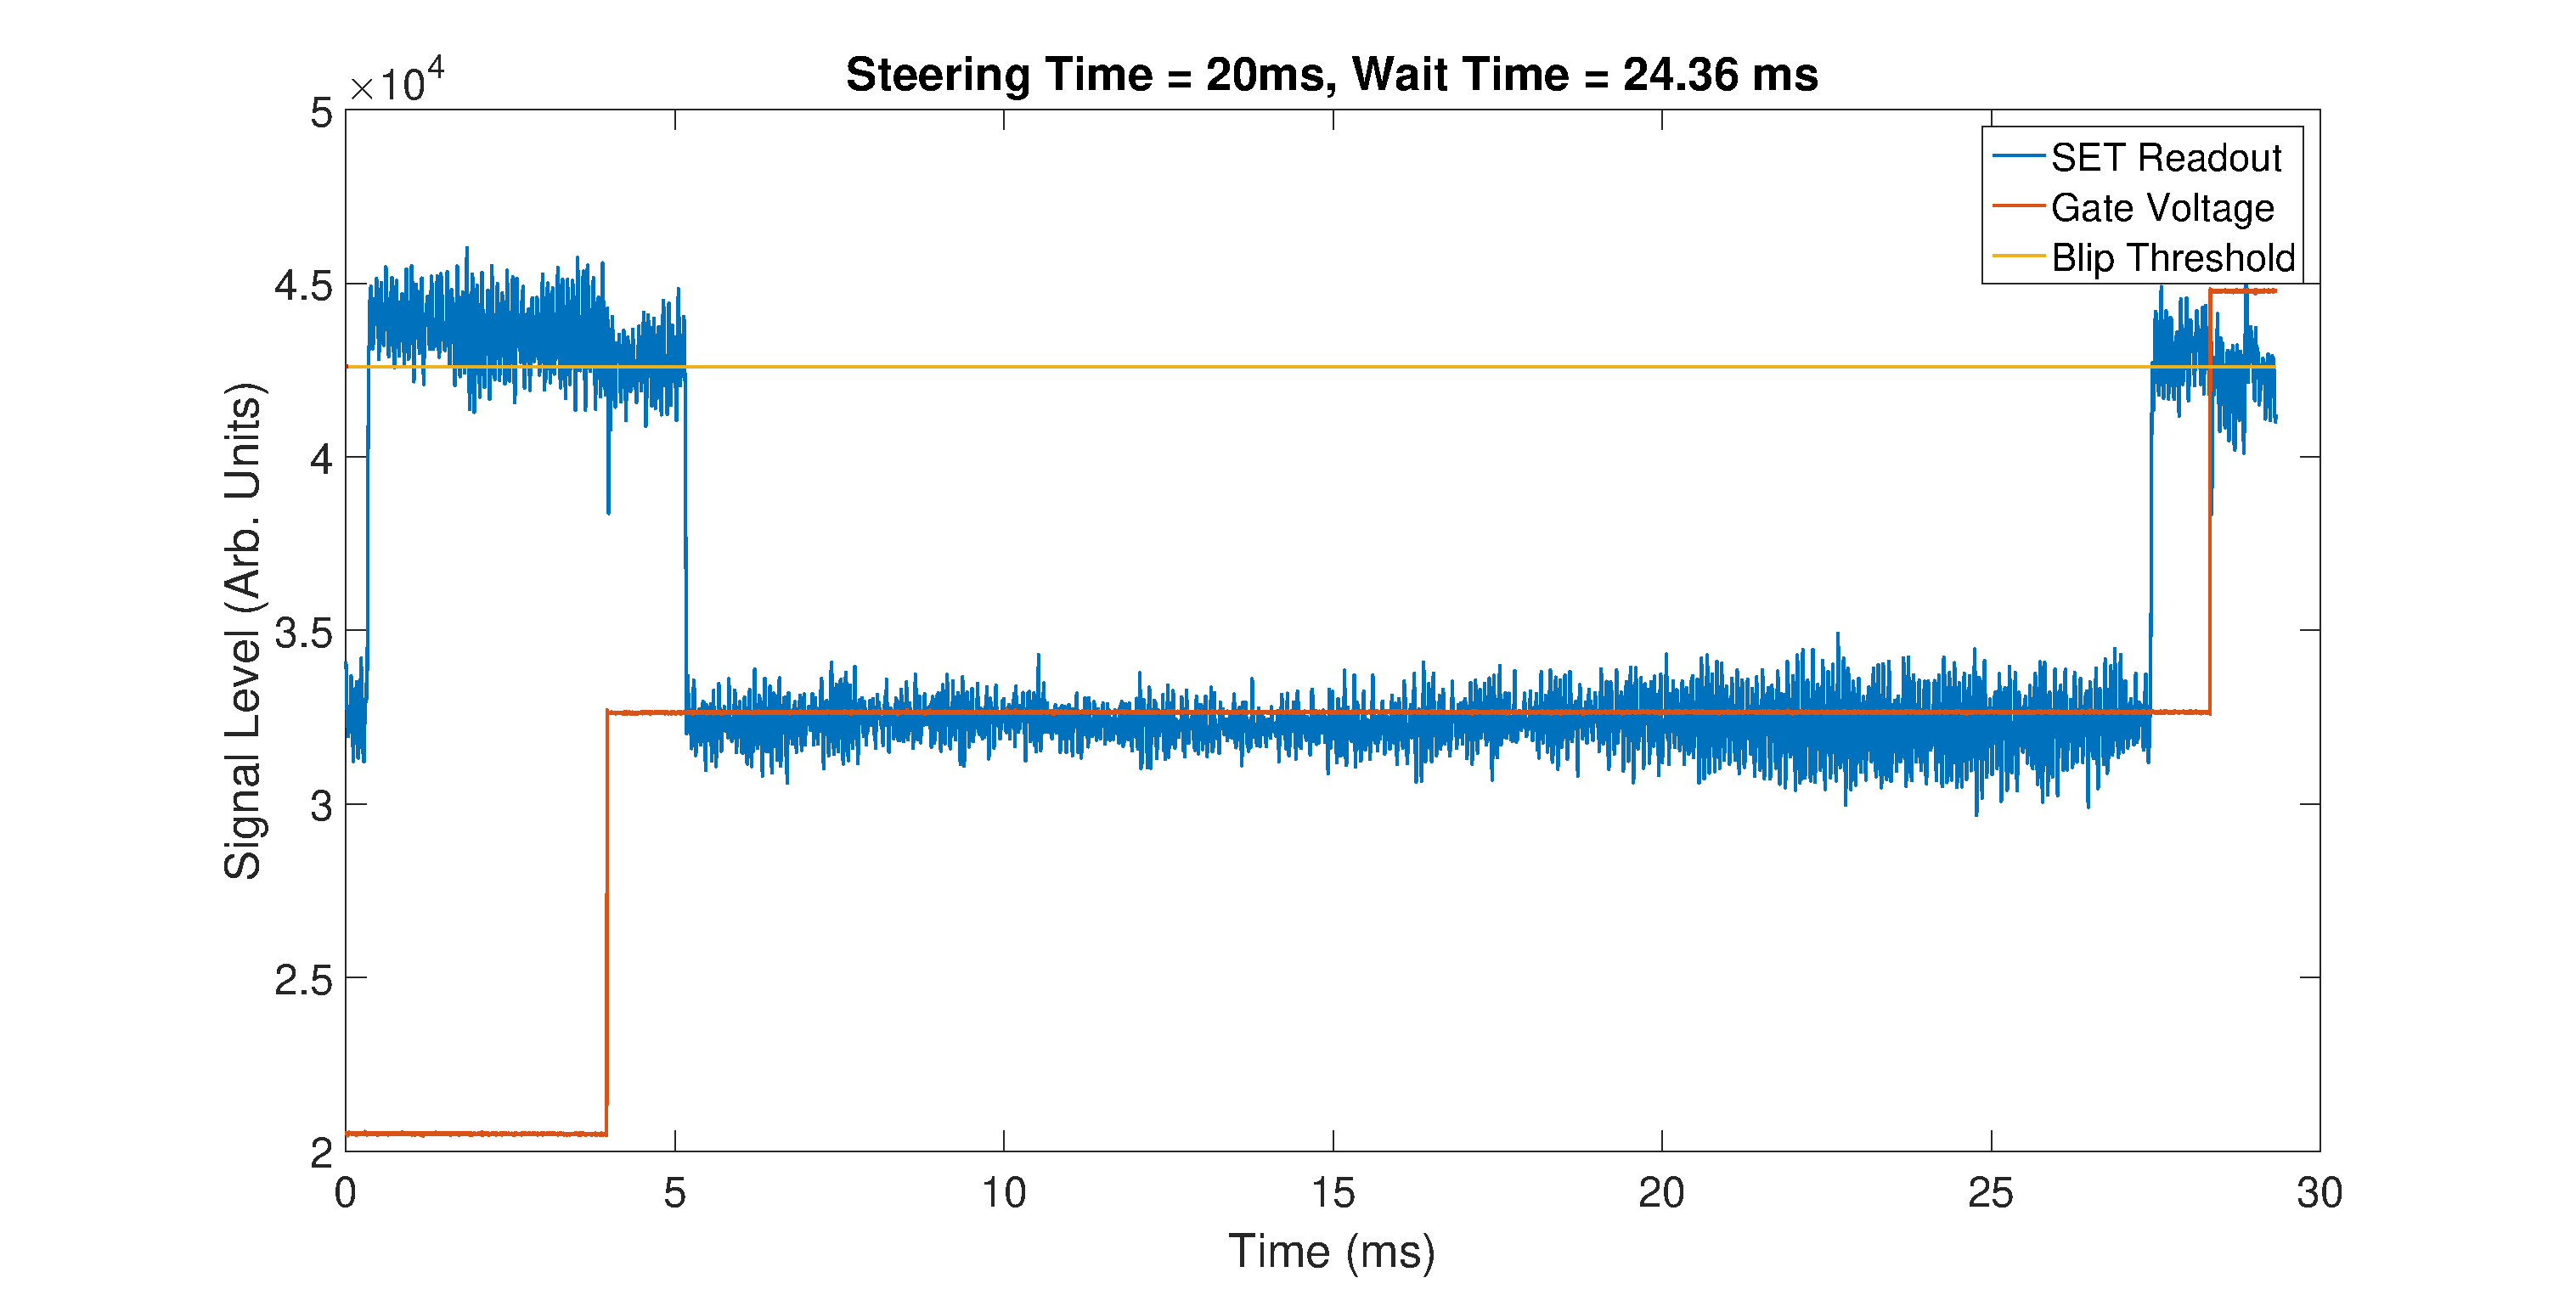
\includegraphics[width=\textwidth]{MATLAB_latency}
		\caption{Improper initialisation occurs due to a latency in the trigger sent by MATLAB.}
		\label{fig::latency}
	\end{figure}
	
	\begin{figure}[htb!]
		\centering
		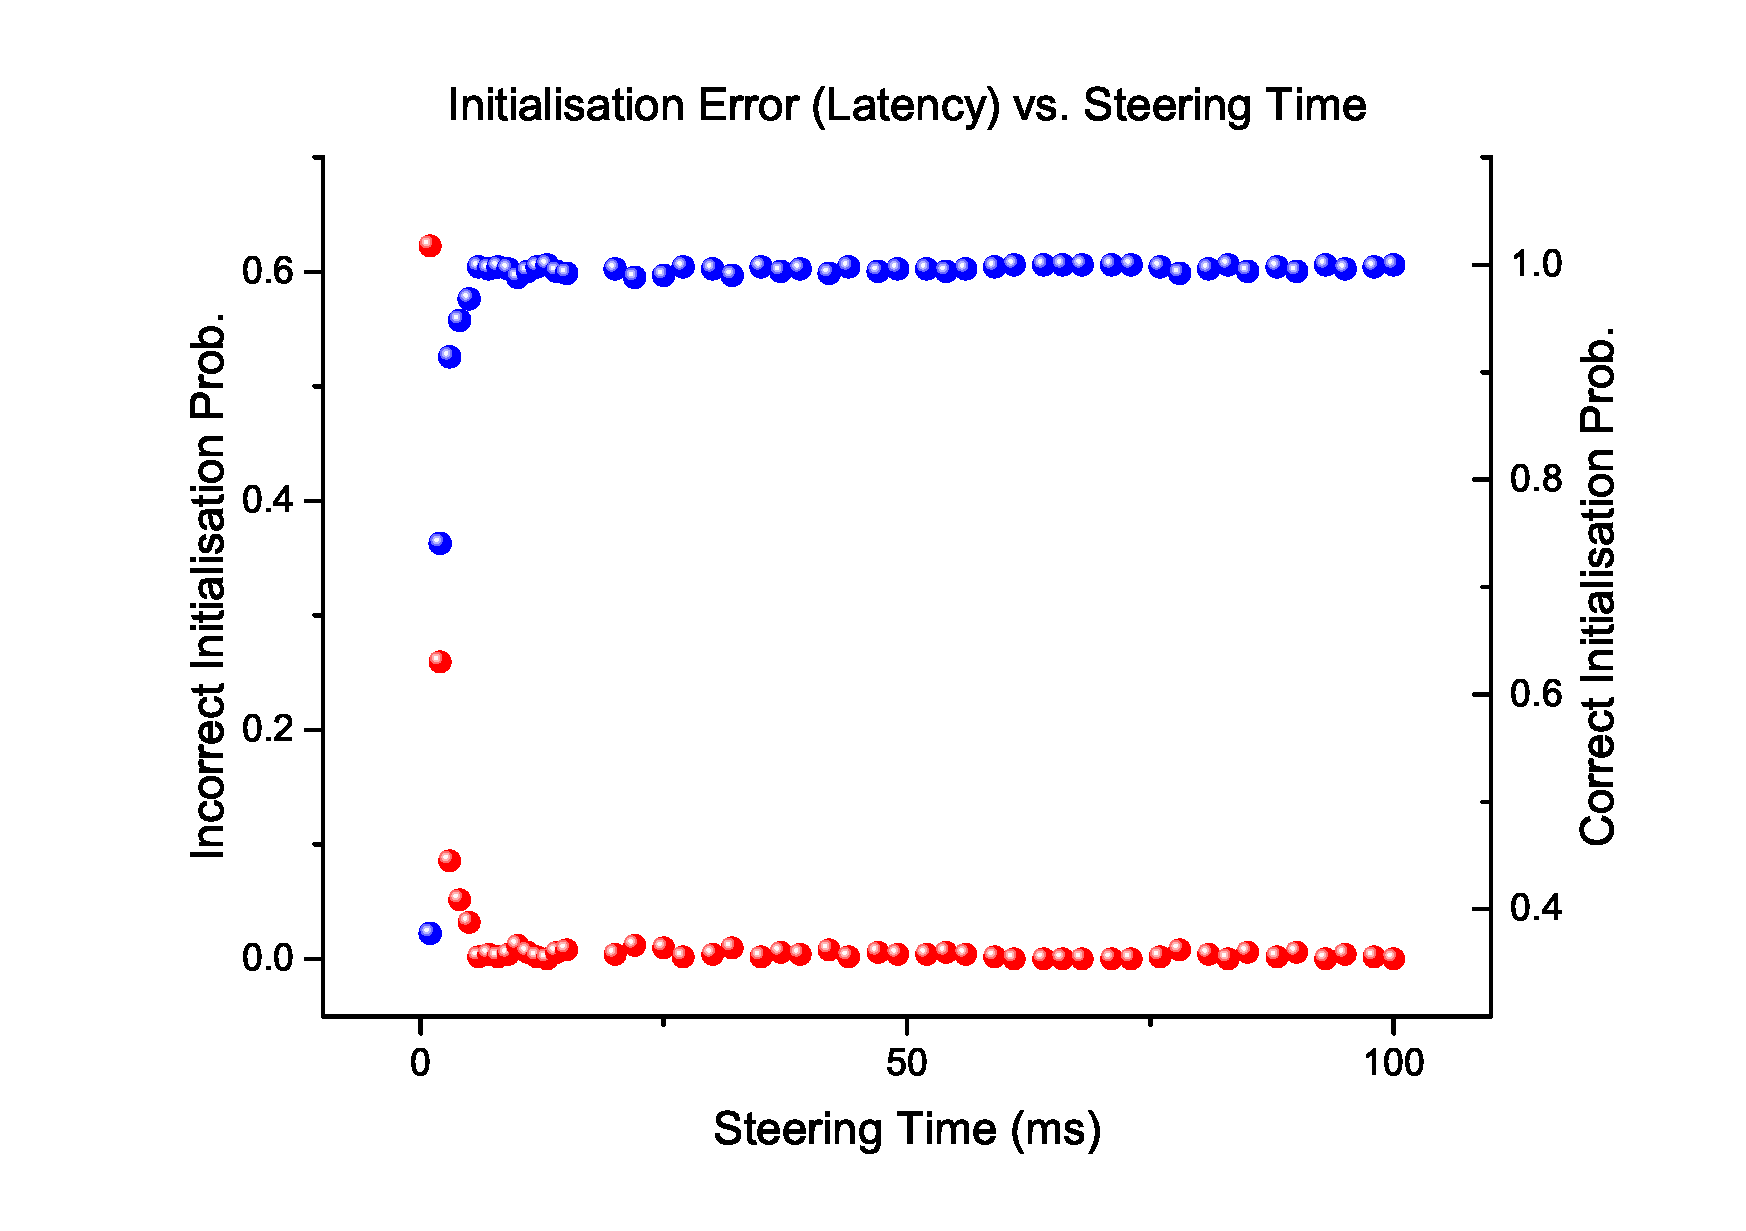
\includegraphics[width=\textwidth]{LatencyErrorFig}
		\caption{Probability of incorrect initialisation with varying steering times.}
		\label{fig::latency_errors}
	\end{figure}
	
	This has been the sole drive for further post-selection in the data, and for low steering times it has a significant effect however with longer steering times, the probability of an electron tunnelling off the donor diminishes, meaning there is a sharp decrease in latency errors. It is evident from the plots that after 6 ms of steering time, the probability of seemingly correct initialisation  is always greater than 98.8\%. Note that this is not a guarantee on the true state of the initialised electron, merely a guarantee that the initialisation scheme has run as expected. This confirms the reliability of a pre-selecting digital feedback loop, and holds room for improvement in mitigating the effect due to latency. The primary result from this analysis is that despite the potential for initialisation errors due to software to hardware latency, it is in fact a rare occurrence. This indicates pre-selection is far superior to post-selecting data that does not fit the required steering time, in terms of data economy. 
	%\todo{find out how much post-selection is done}
	
	There is a potential discrepancy between the observed, correct initialisation and the total experimental fidelity as a function of steering time. As noted in \hyperref[sec::steering]{Section \ref{sec::steering}}, the total fidelity only exceeds 98.8\% after a steering time of approximately 40 ms (Figure \ref{fig::wait_time}, 1.0 T), in contrast to 6 ms noted above. This discrepancy can be quashed when considering longer tunnel times at this magnetic field. While an initialisation may look correct, for small steering times relative to the tunnel time, the spin state will only be steered toward spin-down a small amount. Regardless of the number of correct or incorrect initialisations in this situation, the spin-state is poorly defined and therefore yields a poor total fidelity.
%	\todo{get a value for tunnel time}
	
\pagebreak
\section{Design Improvements}
To improve further on initialisation, this software-defined feedback loop should be shifted into an integrated solution, such as a purpose-built solution with a \gls{mcu} or \gls{fpga}. While an \gls{fpga} would be easy to apply to the problem of detecting blips and measuring time, there is a complexity in integrating an \gls{fpga} based solution with \gls{daq}. 

Data acquisition has been solely performed by a \gls{pcie} connected digitizer card, where data is dumped directly to memory and then saved to a hard-disk. If an \gls{fpga} were to be used in the manner described above, it would either need to introduce a separate \gls{daq} system, where data processed in the \gls{fpga} is collected separately from what is stored on hard-disk, or the introduced \gls{daq} would need to also store its data for analysis.

\begin{figure}[htbp]
	\centering
	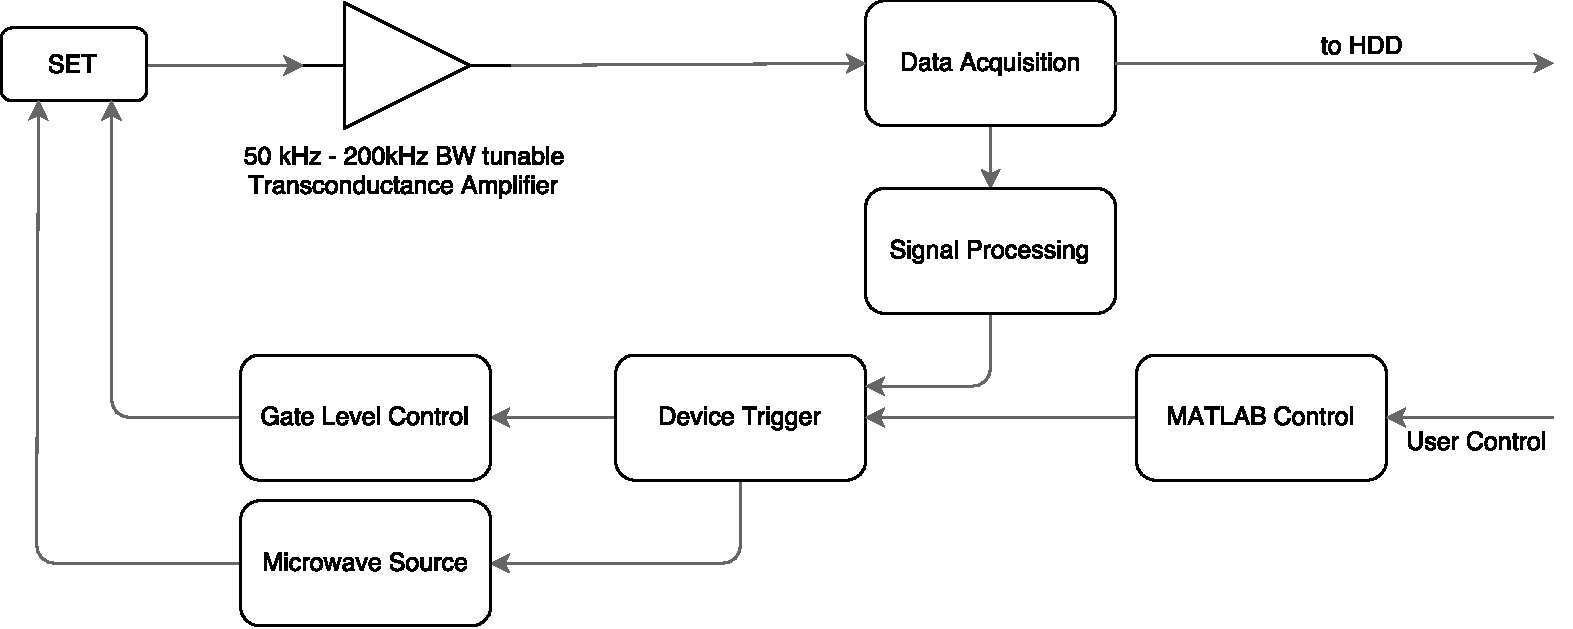
\includegraphics[width=\textwidth]{thesis_redesign_1}
	\caption{An integrated solution which writes data back to disk.}
	\label{fig::redesign_1}
\end{figure}

The first solution holds far more complexity, as it requires designing a system with a \gls{daq} and an \gls{fpga}. This would likely end up using a custom \gls{pcb}, with a special purpose \gls{adc}. The construction and verification of such a device is an undertaking not suited for a research environment where this is not the end product. Similarly, the second solution is not ideal. Storing data from an \gls{fpga} would again require specialised hardware to interface with a hard-disk. 


\begin{figure}[htbp]
	\centering
	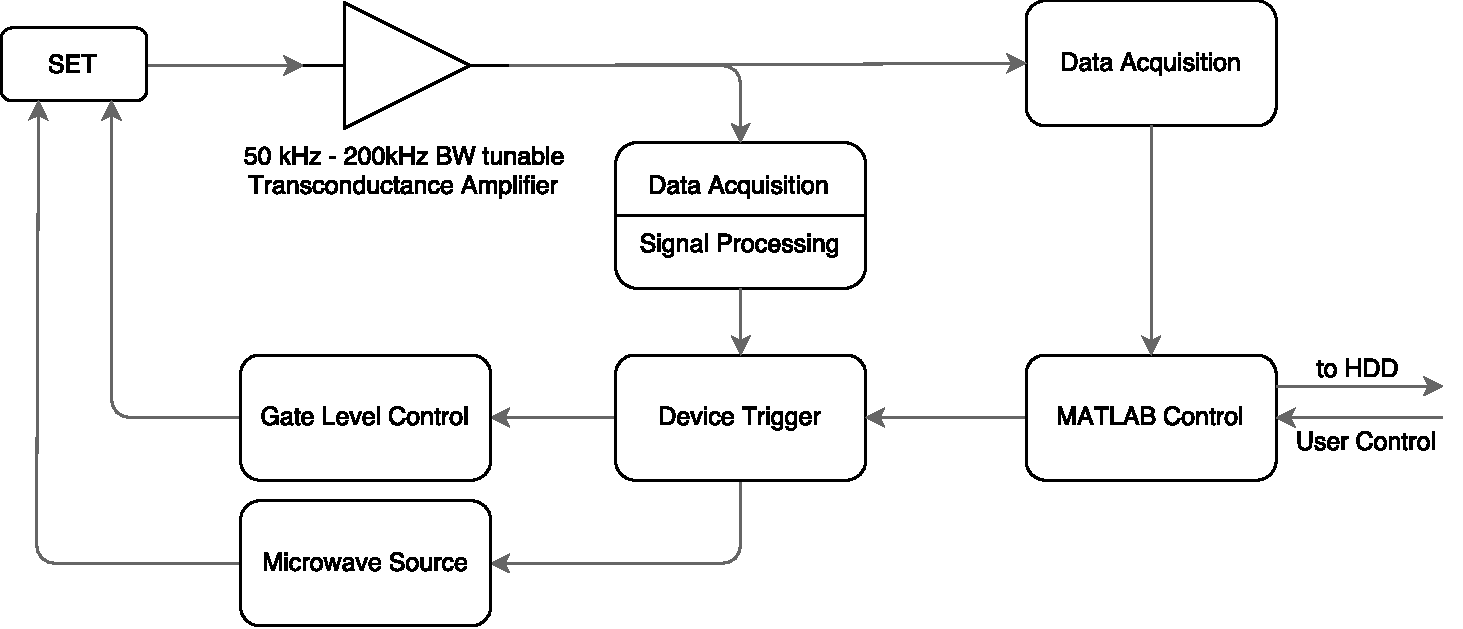
\includegraphics[width=\textwidth]{thesis_redesign_2}
	\caption{An integrated solution which adds a separate data acquisition stage to the feedback loop.}
	\label{fig::redesign_2}
\end{figure}

Ultimately, the desired solution should be integrated in a manner fit for use by non-electronic specialists. As such, a rework of the current set-up will be the preferred method of achieving real-time digital feedback.

The proposed solution is to utilise a \gls{pxie} cabinet with multiple slots to integrate the varied signals and sources we use, including an \gls{awg} and a \gls{daq}. For the problem at hand, there exist combination \gls{fpga} and \gls{daq} cards that allow for pre-processing data and controlling a single digital output, or in more advanced devices, controlling an \gls{awg} via the \gls{fpga}. This solution will be sufficient for performing threshold analysis on a single channel, however it does not make the most of the advantage an \gls{fpga} has over a \gls{mcu}. It has been shown internally in an unpublished form that a \gls{dwt} can detect blips that occur below the threshold level, due to the finite bandwidth of the device and sampling rate of the \gls{daq}.

A Haar \gls{dwt} was used in post-processing data to yield a high-fidelity readout. If this is combined with the initialisation scheme defined in this report, total experiment fidelity is expected to increase much further for lower steering times, and ultimately be more reliable.



\todo[inline]{talk about the viability of such a solution, bring up previous work}
\pagebreak
%\section{Prospective Results}
%\todo[inline]{try and get some simulation results using teh Haar wavelet transform, showing the algorithm run time/latency}
%\pagebreak
\section{Conclusion}
%\todo[inline]{Conclude, like normal}
A quantum computer is the ultimate goal of researchers within \gls{cqc2t}, and devices and experiments are continuously being devised to this end. Devices have been composed of an \gls{set} for spin-dependent readout, a must for a spin-based quantum computer, and experiments are constructed at cryogenic temperatures, and spin qubit manipulation is performed with series of microwave pulses. Before you perform operations on a qubit, it needs to start in a well defined state, and current methods rely on pre-selection of data, based on the criterion of having an electron present at the commencement of the operations. This is an inefficient use of time, and this can be improved by incorporating a digital feedback loop that will perform a strong measurement on the electron spin, and signal the continuation of an experiment.

In my literary review, I have covered some of the fundamental concepts governing the devices being used currently in this research, as well as some other research into the use of digital feedback in quantum systems.
The experimental design explored how the devices were being used together, and where the solution of this thesis will be place in the larger system. It also details some proposed solutions to the lack of digital feedback.
Finally, the prospective plan lists various tasks that are to be completed, from a high-level perspective by the completion of Thesis B.
\pagebreak

\bibliographystyle{ieeetr}	%IEEE style referencing
\bibliography{./src/references}
\pagebreak
\begin{appendices} 
	\section{Glossary}
	\printglossaries
	\pagebreak
	\section{Supplementary Information}
	\paragraph{Big O Notation} describes the limiting behaviour of a function when the argument tends toward infinity.
\label{supp::big_o}
For example, the leading term ($3 x^4$) in the polynomial $p(x) = 3 x^4 + 20 x^2 + 1$, represents the strongest factor that determines the behaviour of the function. As such, we say $p$ has order $\mathcal{O}(n^4)$. Note that we drop any constant multiplier as it doesn't modify the growth or shape of the function.
	\section{MATLAB Software Highlight}
	\lstinputlisting[breaklines=true, language=MATLAB,
					 basicstyle=\footnotesize\ttfamily,
					 numbers=left					
					]{./src/code_digitizer}
\end{appendices}
\end{document}
